\chapter{Extraction de termes-clés}
\label{chap:main-domain_independent_keyphrase_extraction}
  \smallchaptercite{
    [\dots] there is still room for improvement over the task.
  }{
    \newcite{kim2010semeval}
  }

  %-----------------------------------------------------------------------------

  \section{Introduction}
  \label{sec:main:domain_independent_keyphrase_extraction-introduction}
    Dans ce chapitre, nous nous intéressons à la tâche d'extraction automatique
    de termes-clés. Cette tâche consiste à identifier dans un document ses mots
    et expressions qui permettent d'en caractériser le mieux le contenu. C'est
    la catégorie d'indexation par termes-clés la plus étudiée jusqu'à
    maintenant. Elle peut être réalisée de manière non supervisée ou supervisée,
    grâce à la mise en \oe{}uvre d'algorithmes d'ordonnancement par importance
    des mots du document ou grâce à l'entraînement de classificateurs capables
    de déterminer si une unité textuelle est un terme-clé ou non.

    Nous proposons deux contributions à l'extraction automatique de termes-clés.
    Tout d'abord, nous nous intéressons à l'étape préliminaire de sélection des
    termes-clés candidats, puis nous nous intéressons à leur ordonnancement par
    importance. Les méthodes proposées sont non supervisées.

  %-----------------------------------------------------------------------------

  \section{Sélection des termes-clés candidats}
  \label{sec:main:domain_independent_keyphrase_extraction-keyphrase_candidate_selection}
    La sélection des termes-clés candidats établit la liste des termes-clés
    possibles pour un document donné. Bien qu'étudiée en surface, ou de manière
    ad-hoc à une méthode particulière d'extraction de termes-clés, cette étape
    est critique. Si elle ne sélectionne pas
    suffisamment de candidats, alors la performance maximale pouvant être
    atteinte pour l'extraction de termes-clés est faible et, au contraire, si
    elle sélectionne un nombre important de candidats, alors elle augmente le
    risque de sélectionner des candidats erronéspouvant dégrader la performance
    d'une méthode d'extraction de termes-clés~\cite{hasan2014state_of_the_art}.
    De nombreux travaux ont montré que les groupes nominaux, souvent
    approximés par les séquences de noms et d'adjectifs (\texttt{/(N|A)+/}),
    forment de bons termes-clés candidats et sont très proches des termes-clés
    de-
    référence~\cite{barker2000nounphrasehead,hulth2003keywordextraction,wan2008expandrank}.

    Dans notre travail, nous remettons en question la sélection systématique
    d'un adjectif apposé à un groupe nominal. En nous appuyant sur une analyse
    linguistique des termes-clés de trois collections de données en français et
    en anglais, nous proposons une méthode qui juge si un adjectif apporte du
    sens bénéfique à la caractérisation du contenu du document, auquel cas il
    est sélectionné avec le groupe nominal qu'il modifie, ou s'il est superflu,
    auquel cas le groupe nominal seul est sélectionné comme terme-clé candidat.
    Deux évaluations montrent le bien fondé de cette méthode~: l'une
    intrinsèque, l'autre extrinsèque. L'évaluation intrinsèque compare la
    qualité de l'ensemble de termes-clés candidats sélectionnés par notre
    méthode à ceux sélectionnés par les méthodes les plus utilisées (sélection
    des n-grammes, des \textit{chunks} nominaux ou des \texttt{/(N|A)+/})~;
    l'évaluation extrinsèque compare l'impact de notre méthode de sélection sur
    deux méthodes d'extraction de termes-clés à celui des méthodes de sélection
    les plus utilisées.

    \subsection{Analyse des propriétés linguistiques des termes-clés}
    \label{subsec:main:domain_independent_keyphrase_extraction-keyphrase_candidate_selection-analysis_of_keyphrase_properties}
      Afin de sélectionner plus finement les termes-clés candidats, nous
      extrayons et analysons des statistiques concernant les termes-clés~: leur
      taille (en nombre de mots) et la catégorie grammaticale des mots qui les
      composent. Cela nous permet de confirmer les observations faites dans les
      travaux précédents et d'en inférer de nouvelles, axées sur la catégorie
      grammaticale des mots des termes-clés.

      Notre analyse couvre les deux langues de nos ressources~: français et
      anglais. Elle se porte sur les collections \textsc{De}ft (français),
      \textsc{Duc} (anglais) et SemEval (anglais). Dans le but de ne pas biaiser
      les résultats des évaluations de ce travail, l'analyse est effectuée sur
      un sous-ensemble de ces collections. Pour permettre des comparaisons avec
      d'autres travaux, les évaluations sont réalisées sur les ensembles de
      test de nos collections et l'analyse est donc réalisée sur les ensembles
      normalement destinés à l'apprentissage. \textsc{Duc} n'étant pas réparti
      en plusieurs sous-ensembles, nous utilisons 208 documents pour l'analyse
      et 100 pour les évaluations.

      \subsubsection{Analyse surfacique}
      \label{subsubsec:main:domain_independent_keyphrase_extraction-keyphrase_candidate_selection-analysis_of_keyphrase_properties-shalow_analysis}
      Le tableau~\ref{tab:candidate_selection-train_stats} montre la
      proportion de termes-clés uni-grammes, bi-grammes et tri-grammes, ainsi
      que la proportion de termes-clés multi-mots contenant au moins un mot
      appartenant à l'une des sept catégories grammaticales que nous observons
      en leur sein\footnote{ Nous nous focalisons sur les expressions
      (termes-clés multi-mots), car nous avons observé que la quasi totalité des
      termes-clés composés d'un unique mot sont des noms. }~: nom commun, nom
      propre, adjectif, verbe, adverbe, préposition et déterminant. Pour obtenir
      ces informations, les termes-clés ont été automatiquement segmentés en
      mots et étiquetés grammaticalement à l'aide des outils utilisés pour
      prétraiter les collections de données (cf
      section~\ref{sec:main-data_description-preprocessing}
      page~\pageref{sec:main-data_description-preprocessing}), puis manuellement
      corrigés.
      \begin{table}[!h]
        \centering
        \begin{tabular}{ll|ccc}
          \toprule
          & & \textbf{\textsc{Duc}} \textit{(en)} & \textbf{SemEval} \textit{(en)} & \textbf{\textsc{Deft}} \textit{(fr)}\\
          \hline
          \multicolumn{2}{l|}{\textbf{Taux (en \%) de termes-clés~:}}\\
          & Uni-grammes & 17,1 & 20,2 & 60,2\\
          & Bi-grammes & 60,8 & 53,4 & 24,5\\
          & Tri-grammes & 17,8 & 21,3 & 8,8\\
          \hline
          \multicolumn{2}{l|}{\textbf{Taux (en \%) de termes-clés}} & & &\\
          \multicolumn{2}{l|}{\textbf{contenant au moins un(e)~:}} & & &\\
          & Nom commun & 94,5 & 98,7 & 93,1\\
          & Nom propre & 17,1 & $~~$4,3 & $~~$6,9\\
          & Adjectif & 50,0 & 50,2 & 65,5\\
          & Verbe & $~~$1,0 & $~~$4,0 & $~~$1,0\\
          & Adverbe & $~~$1,6 & $~~$0,7 & $~~$1,3\\
          & Préposition & $~~$0,3 & $~~$1,5 & 31,2\\
          & Déterminant & $~~$0,0 & $~~$0,0 & 20,4\\
          \bottomrule
        \end{tabular}
        \caption{Statistiques concernant les termes-clés de référence des
                 collections \textsc{Deft}, SemEval et \textsc{Duc}
                 \label{tab:candidate_selection-train_stats}}
      \end{table}

      Concernant la taille des termes-clés de référence, les uni-grammes,
      bi-grammes et tri-grammes couvrent plus de 90~\% des termes-clés de
      références. En français, ce sont les uni-grammes qui sont les plus
      utilisés, suivis par les bi-grammes, tandis qu'en anglais, ce sont les
      bi-grammes qui sont les plus employés, avec des proportions équivalentes
      d'uni-grammes et de tri-grammes. Ces premières observations font écho à
      celles que nous trouvons dans la littérature. Nous en concluons qu'il
      s'agit de propriétés stables des termes-clés. Une approche raisonable peut
      donc se restreindre aux $\{1..3\}$-grammes, à l'instar de celle de
      \newcite{witten1999kea}.

      Concernant les catégories des mots que contiennent les termes-clés de
      référence, nous observons que la quasi-totalité des termes-clés
      contiennent un nom (ce sont majoritairement des groupes nominaux) et
      que la moitié d'entre eux est modifiée par un adjectif. Les autres
      catégories de mots, comme le verbe et l'adverbe sont très peu utilisées.
      L'usage de ces dernières au sein de termes-clés semble être exceptionnel.
      Les déterminants et prépositions ont un usage presque exclusivement
      français. En anglais, les modifications nominales (par exemple,
      \textit{\og{}nature conservation\fg{}} -- \og{}conservation de la
      nature\fg{}) sont préférées aux formes syntagmatiques (par exemple~:
      \textit{\og{}conservation of nature\fg{}} -- \og{}conservation de la
      nature\fg{}).

      \subsubsection{Analyse des adjectifs}
      \label{subsubsec:main:domain_independent_keyphrase_extraction-keyphrase_candidate_selection-analysis_of_keyphrase_properties-adjective_analysis}
      Après le nom et le nom propre, c'est l'adjectif qui est le plus utilisé.
      Nous analysons plus finement sa nature et examinons les trois catégories
      d'adjectifs suivantes~: relationnel, composé complexe et qualificatif.
      
      Un adjectif relationnel est un adjectif
      dénominal~\cite{bally1944linguistiquegeneraleetlinguistiquefrancaise}. Il
      est dérivé d'un nom (par exemple~: l'adjectif relationnel
      \og{}culturel\fg{} est dérivé du nom \og{}culture\fg{}) pour lequel il
      établit une relation équivalente à celle exprimée par le complément du nom
      (par exemple~: \og{}héritage culturel\fg{} équivaut à \og{}héritage de la
      culture\fg{}). Caractéristique du discours du
      spécialiste~\cite{maniez2009denominaladjectives}, l'adjectif relationnel
      sert de modificateur dans les titres de catégories, telles que celles de
      Wikipedia (par exemple \og{}héritage
      culturel\fg{}\footnote{\url{http://en.wikipedia.org/wiki/Category:Cultural_heritage}}),
      qui constituent de bons termes-clés
      candidats~\cite{medelyan2008smalltrainingset,eichler2010keywe}. Par
      transitivité, l'adjectif relationnel semble donc être un modificateur qui
      apporte du sens bénéfique à la caractérisation  de tout ou partie du
      contenu d'un document.
      
      Un adjectif composé complexe est un adjectif constitué de plusieurs mots,
      souvent délimités graphiquement par un trait d'union (par exemple,
      \og{}socio-éducatif\fg{}). L'adjectif composé complexe contribue avec
      précision et concision à la caractérisation du nom qu'il modifie (par
      exemple, \og{}activité socio-éducative\fg{} hyponyme de
      \og{}activité\fg{}). Pour cette raison, nous pensons qu'il est utile pour
      caractériser tout ou partie du contenu d'un document. De plus, la
      composition adjectivale est l'un des processus privilégiés pour la
      formation de néologismes\footnote{Néologisme~: mot nouveau, emprunt récent
      à une autre langue ou nouvelle emploi d'un mot déjà existant (nouvelle
      acception).}~\cite{boughedaoui1997adjectifscomposes}.

      Un adjectif qualificatif est un adjectif qui donne une qualification à un
      nom. Il désigne la qualité ou la manière d'être (par exemple,
      \og{}grand\fg{}) de ce dernier. Cette catégorie d'adjectifs est la plus
      courante. L'ensemble des cas d'utilisation des adjectifs qualificatifs est
      moins restreint que celui des adjectifs relationnels et composés
      complexes. Nous faisons donc l'hypothèse qu'un adjectif appartenant à
      cette catégorie n'est pas toujours utile à la caractérisation du contenu
      d'un document.
      
      ~\\Pour détecter les adjectifs relationnels, nous utilisons une technique
      simple, adaptée (ou adaptable) à plusieurs langues et ne requérant pas
      nécessairement de ressources linguistiques finies.

      Dans un premier temps, les adjectifs relationnels sont détectés avec une
      base de données lexicale. Pour le français, nous utilisons la base
      WoNeF~\cite{pradet2013wonef}. Pour l'anglais, nous
      utilisons la base  WordNet~\cite{miller1995wordnet}. WoNeF est issue de
      WordNet, ses entrées ont été obtenues par traduction de WordNet. Pour
      savoir si un adjectif est relationnel, nous utilisons la propriété
      \texttt{[PERTAINYM]} de WordNet et son équivalent \texttt{[DERIVED]} dans
      WoNeF.

      Dans un second temps, les adjectifs relationnels qui ne sont pas présents
      dans la base de données lexicale sont détectés à l'aide de leur
      suffixe~\cite{dubois1999derivation}. Une liste des suffixes les plus
      productifs pour les adjectifs relationnels est utilisée pour identifier
      les adjectifs relationnels potentiels. En français, les suffixes les plus
      productifs sont \textit{-ain}, \textit{-aire}, \textit{-al}, \textit{-el},
      \textit{-esque}, \textit{-estre}, \textit{-eux}, \textit{-ien},
      \textit{-ier}, \textit{-if}, \textit{-il}, \textit{-in}, \textit{-ique},
      \textit{-ois}, et
      \textit{-é}~\cite{harastani2013relationaladjectivetranslation}~; en
      anglais, les suffixes utilisés sont \textit{-al}, \textit{-ant},
      \textit{-ary}, \textit{-ic}, \textit{-ous} et
      \textit{-ive}~\cite{grabar2006terminologystructuring}.

      La détection des adjectifs relationnels, telle que nous la réalisons,
      n'est pas exacte. En effet, les adjectifs qualificatifs et/ou
      dénominaux se terminant par un suffixe d'adjectif relationnel sont
      détectés comme relationnels, et les adjectifs à usage tantôt qualificatif,
      tantôt relationnel selon le contexte~\cite{maniez2009denominaladjectives}
      sont toujours détectés comme relationnels. Dans la littérature, les
      approches pour identifier les adjectifs relationnels (dans le cadre de
      l'extraction terminologique) reposent sur une analyse en
      corpus~\cite{daille2000relationaladjectives,maniez2005automaticrelationaladjectiveidentification,harastani2013relationaladjectivetranslation},
      où il s'agit notamment de trouver des paraphrases avec un complément de
      nom. Dans le contexte de l'extraction de termes-clés, où de larges corpus
      ne sont pas toujours disponibles, les paraphrases ne sont pas toutes
      présentes et de telles approches ne sont pas applicables. De plus,
      \newcite{harastani2013relationaladjectivetranslation} montrent qu'une
      approche comme la notre reste une alternative viable.

      ~\\Pour déterminer si un adjectif est composé, nous regardons s'il possède
      un trait d'union. Le trait d'union est l'unique marque explicite de
      composition en français et en anglais, et son usage est le procédé le plus
      productif. Néanmoins, il existe deux autres procédés que nous ne traitons
      pas~: les mots qui constituent l'adjectif composé sont parfois séparés
      par un espace ou concaténés sans marque explicite.

      ~\\Le tableau~\ref{tab:candidate_selection-adjective_categories} donne le
      taux d'adjectifs, par catégorie, dans les termes-clés de référence. Nous
      observons que la majorité de ces adjectifs sont relationnels, ce qui
      conforte notre hypothèse que les adjectifs relationnels sont des
      modificateurs utiles pour les termes-clés. Ceci est confirmé par le
      tableau~\ref{tab:candidate_selection-best_patterns} qui montre que l'un
      des patrons grammaticaux les plus productifs de termes-clés représente un
      nom modifié par un adjectif relationnel. Le cas des adjectifs composés
      complexes est moins marqué. Ils sont peu employés par rapport aux
      adjectifs relationnels et aux adjectifs qualificatifs. Ces derniers, quant
      à eux, ont un emploi non négligeable, en particulier en anglais où ils
      font partie de l'un des patrons grammaticaux les plus productifs de
      termes-clés (cf tableau~\ref{tab:candidate_selection-best_patterns}).
      \begin{table}[!ht]
        \centering
          \begin{tabular}{l|ccc}
            \toprule
            & \textbf{\textsc{Duc}} \textit{(en)} & \textbf{SemEval} \textit{(en)} & \textbf{\textsc{De}ft} \textit{(fr)}\\
            \hline
            Adjectifs relationnels \hfill(\%) & 53,1 & 43,6 & 87,1\\
            Adjectifs composés complexes \hfill(\%) & 10,6 & 16,4 & $~~$3,3\\
            Adjectifs qualificatifs \hfill(\%) & 36,3 & 40,0 & $~~$9,6\\
            \bottomrule
        \end{tabular}
        \caption{Taux d'adjectifs, par catégorie (relationnel, composé complexe
                 ou qualificatif), au sein des termes-clés de référence}
                 \label{tab:candidate_selection-adjective_categories}
      \end{table}

      Le tableau~\ref{tab:candidate_selection-adjective_categories_in_documents}
      montre le taux d'adjectifs, par catégorie, dans les documents. En
      comparant les taux présentés dans le
      tableau~\ref{tab:candidate_selection-adjective_categories} à ceux du
      tableau~\ref{tab:candidate_selection-adjective_categories_in_documents}
      nous pouvons déduire le degré d'ambigüité d'un adjectif en tant que
      modificateur utile dans un terme-clé. Ainsi, ce tableau montre qu'il y a
      moins d'ambigüités quant à l'appartenance d'un adjectif relationnel ou
      composé à un terme-clé, car ces deux catégories d'adjectifs sont nettement
      moins utilisées dans les documents que dans les termes-clés de référence.
      À l'inverse, les adjectifs qualificatifs ont un très fort usage dans les
      documents et il y a donc plus d'ambigüité quant à leur nécessité en tant
      que modificateur dans un terme-clé.
      \begin{table}[!h]
        \centering
          \begin{tabular}{l|ccc}
            \toprule
            & \textbf{\textsc{Duc}} \textit{(en)} & \textbf{SemEval} \textit{(en)} & \textbf{\textsc{De}ft} \textit{(fr)}\\
            \hline
            Adjectifs relationnels \hfill(\%) & 29,9 & 30,7 & 61,9\\
            Adjectifs composés complexes \hfill(\%) & $~~$8,8 & $~~$7,9 & $~~$0,4\\
            Adjectifs qualificatifs \hfill(\%) & 61,3 & 61,4 & 37,7\\
            \bottomrule
        \end{tabular}
        \caption{Taux d'adjectifs, par catégorie (relationnel, composé complexe
                 ou qualificatif), au sein des documents}
                 \label{tab:candidate_selection-adjective_categories_in_documents}
      \end{table}

      \begin{table}[!h]
        \centering
        \begin{tabular}{r@{~}|@{~}l@{~}l@{~}l@{~}llr}
          \toprule
          \multicolumn{1}{r@{~}|@{~}}{} & \multicolumn{4}{@{}l}{\textbf{Pattern}} & \textbf{Example} & \textbf{\%}\\
          \hline
          \multirow{5}{*}{\begin{sideways}\textbf{Français}\end{sideways}}
          & \texttt{Nc} & \texttt{Ar} & & & \TODO{exemple} & 46,4\\
          & \texttt{NC} & \texttt{Sp} & \texttt{D} & \texttt{Nc} & \TODO{exemple} & 12,5\\
          & \texttt{Nc} & \texttt{Sp} & \texttt{Nc} & & \TODO{exemple} & $~~$8,2\\
          & \texttt{Nc} & \texttt{A} & & & \TODO{exemple} & $~~$4,3\\
          & \texttt{Np} & \texttt{Np} & & & \TODO{exemple} & $~~$3,0\\
          \hline
          \multirow{5}{*}{\begin{sideways}\textbf{Anglais}\end{sideways}}
          & \texttt{Nc} & \texttt{Nc} & & & \TODO{exemple} & 32,5\\
          & \texttt{Ar} & \texttt{Nc} & & & \TODO{exemple} & 15,1\\
          & \texttt{A} & \texttt{Nc} & & & \TODO{exemple} & $~~$9,5\\
          & \texttt{Nc} & \texttt{Nc} & \texttt{Nc} & & \TODO{exemple} & $~~$5,3\\
          & \texttt{Ac} & \texttt{Nc} & & & \TODO{exemple} & $~~$4,9\\
          \bottomrule
        \end{tabular}
        \caption[
          Patrons grammaticaux les plus fréquents parmi les termes-clés
          français et anglais
        ]{
          Patrons grammaticaux les plus fréquents parmi les termes-clés
          français et anglais. Les classes grammaticales sont exprimées au
          format Multext~\cite{ide1994multext}, sauf \texttt{Ar} et \texttt{Ac}
          qui représentent, respectivement, un adjectif relationnel et un
          adjectif composé.
          \label{tab:candidate_selection-best_patterns}
        }
      \end{table}

      \subsubsection{Bilan}
      \label{subsubsec:main:domain_independent_keyphrase_extraction-keyphrase_candidate_selection-analysis_of_keyphrase_properties-conclusion}
        Cette analyse des propriétés linguistiques des termes-clés montre que ce
        sont majoritairement des groupes nominaux de petite taille.
        La modification adjectivale est très utilisée (dans plus de la moitié
        des cas) pour rendre plus spécifique les termes-clés. Les adjectifs
        utilisés comme modificateurs au sein des termes-clés peuvent être de
        différente nature, les plus remarquables étant les adjectifs
        relationnels, de par leur définition et de par leur très faible
        ambigüité observée quant à leur appartenance à un terme-clé.
        Inversement, les adjectifs qualificatifs sont les plus courants et ne
        sont pas nécessairement utiles au sein de termes-clés. Ils doivent être
        retenus comme modificateusr dans les termes-clés candidats que s'ils
        respectent certaines conditions (définis ci-après).

    \subsection{Sélection fine des termes-clés candidats}
    \label{subsec:main:domain_independent_keyphrase_extraction-keyphrase_candidate_selection-modifiers_filtering}
      Pour sélectionner les termes-clés candidats, nous proposons une méthode
      explorant les propriétés linguistiques remarquables des termes-clés. Cette
      méthode commence par présélectionner les termes-clés candidats à l'aide
      d'un patron grammatical, puis elle filtre les adjectifs qualificatifs dans
      certaines conditions.

      \subsubsection{Présélection des termes-clés candidats}
      \label{subsubsec:main:domain_independent_keyphrase_extraction-keyphrase_candidate_selection-modifiers_filtering-candidate_pre_selection}
        L'étape de présélection des candidats utilise un patron grammatical
        défini sous la forme d'une expression rationnelle. Celui-ci est appliqué
        aux catégories grammaticales des séquences de mots adjacents dans le
        document et sélectionne celles qui le respectent. Ce patron est
        gourmand, c'est-à-dire qu'il capture les plus longues séquences
        possibles sans produire de candidats qui se recouvrent dans le texte
        (comme c'est le cas avec les n-grammes). Il permet ainsi de diminuer le
        risque d'extraire des termes-clés
        redondants~\cite{hasan2014state_of_the_art}.

        D'après nos observations, seuls les noms, les adjectifs, les
        prépositions et les déterminants sont utiles pour sélectionner les
        termes-clés candidats en permettant une performance maximale
        quasi-optimale. Dans le cas de l'anglais, les prépositions et les
        déterminants sont en proportions très faibles et peuvent donc ne pas
        être considéré lors de la définition du patron grammatical. Dans le cas
        du français, les prépositions et les déterminants apparaissent au sein
        de plus de 30~\% des termes-clés de référence. Notre étude se portant
        sur les adjectifs uniquement, nous faisons le choix de ne pas considérer
        ces deux classes grammaticales lors de la définition du patron de
        présélection des termes-clés candidats. Pour l'adjectif, nous nous
        appuyons sur les patrons grammaticaux les plus productifs de termes-clés
        du tableau~\ref{tab:candidate_selection-best_patterns} et décidons de
        limiter le nombre d'adjectifs à un pour le français et
        l'anglais\footnote{En français et en anglais, 3,3~\% et 5,3~\% des
        termes-clés contiennent plus d'un adjectif, respectivement.}.
        
        Pour le français, nous définissons le patron \texttt{/N+ A?/}, qui
        accepte une séquence de noms (ou noms propres) se terminant
        optionnellement par un adjectif. En français, l'adjectif peut être soit
        antéposé, soit postposé. Le patron que nous avons défini n'accepte que
        les adjectifs postposés pour deux raisons. La première raison est que
        les adjectifs relationnels, que nous jugeons les
        plus utiles au sein des termes-clés, sont toujours postposés. La seconde
        raison est que l'adjectif antéposé ne fait pas partie des patrons les
        plus productifs de termes-clés\footnote{En français, seulement 0,7~\%
        des termes-clés commencent par un adjectif.} (cf
        tableau~\ref{tab:candidate_selection-best_patterns}).
        
        Pour l'anglais, nous définissons le parton \texttt{/A? N+/}, qui accepte
        une séquence de noms (ou noms propres) modifiée optionnellement par un
        adjectif antéposé. En anglais, tous les adjectifs sont antéposés. Ce
        patron ne filtre donc aucun adjectif à cette étape de présélection.

      \subsubsection{Filtrage des adjectifs superflus}
      \label{subsubsec:main:domain_independent_keyphrase_extraction-keyphrase_candidate_selection-modifiers_filtering-adjective_filtering}
        L'orsqu'un candidat contient un adjectif, cette étape juge s'il doit
        faire partie du terme-clé candidat ou non, auquel cas il  en est retiré.
        Sur la base de notre analyse, les adjectifs relationnels et composés
        complexes sont systématiquement jugés utiles. Seuls les adjectifs
        qualificatifs font l'objet d'une prise de décision.

        Pour décider si un adjectif qualificatif apporte du sens utile au groupe
        nominal qu'il modifie dans le terme-clé candidat, nous comparons les
        usages respectifs du candidat avec l'adjectif et sans l'adjectif. Notre
        intuition est qu'un adjectif est superflu (inutile) s'il modifie un
        groupe nominal qui est utilisé de manière autonome (sans l'adjectif) un
        nombre significatif de fois. Concrètement, si le groupe nominal occure
        plus souvent sans l'adjectif qu'avec l'adjectif, alors ce dernier est
        jugé inutile et est donc retiré du terme-clé candidat.

        L'algorithme~\ref{algo:candidate_pruning} résume le fonctionnement de
        notre méthode de sélection des termes-clés candidats. Les lignes
        \ref{algo:line:start_preselection} à \ref{algo:line:end_preselection}
        concernent la présélection des candidats et les lignes
        \ref{algo:line:start_filtering} à \ref{algo:line:end_filtering}
        identifient et filtrent les adjectifs qualificatifs superflus.
        \begin{algorithm}
          \SetKwInOut{kwInput}{Entrée}
          \SetKwInOut{kwOutput}{Sortie}
          \SetKwFor{For}{Pour chaque}{faire}{}
          \SetKwIF{If}{ElseIf}{Else}{Si}{alors}{Sinon si}{Sinon}{}
          \SetKw{KwRet}{Retourner}
          \DontPrintSemicolon{}

          \kwInput{document}
          \kwOutput{candidats}
          \BlankLine

          patron $\leftarrow$ Nil\;\label{algo:line:start_preselection}
          \If{\textnormal{document.langue = "francais"}}{
            patron $\leftarrow$ \texttt{/N+ A?/}\;
          }\Else{
            \If{\textnormal{document.langue = "anglais"}}{
              patron $\leftarrow$ \texttt{/A? N+/}\;
            }
          }

          candidats $\leftarrow$ \{\}\;
          candidats\_preliminaires $\leftarrow$ preselection(document, patron)\;\label{algo:line:end_preselection}

          \For{\textnormal{cdt} $\in$ \textnormal{candidats\_preliminaires}}{\label{algo:line:start_filtering}
            \If{$\exists{}\textnormal{mot} \in$ \textnormal{cdt},
            \textnormal{estAdjectif(mot)} $\wedge$ $\overline{\textnormal{estRelationnel(mot)}}$ $\wedge$ $\overline{\textnormal{estCompose(mot)}}$}{
              tete\_cdt $\leftarrow$ cdt$_{\setminus\{\textnormal{mot}\}}$\;
              freq\_cdt $\leftarrow$ \textnormal{document.conter(cdt)}\;
              freq\_tete\_cdt $\leftarrow$ \textnormal{document.conter(tete\_cdt)} $-$ freq\_cdt\;
              \If{\textnormal{freq\_cdt} $>$ \textnormal{freq\_tete\_cdt}}{
                candidats $\leftarrow$ candidats $\cup$ \{cdt\}\;
              }\Else{
                candidats $\leftarrow$ candidats $\cup$ \{tete\_cdt\}\;
              }
            }\Else{
              candidats $\leftarrow$ candidats $\cup$ \{cdt\}\;
            }
          }\label{algo:line:end_filtering}

          \caption{Sélection fine des termes-clés candidats
                   \label{algo:candidate_pruning}}
        \end{algorithm}

    \subsection{Évaluation}
    \label{subsec:main:domain_independent_keyphrase_extraction-keyphrase_candidate_selection-evaluation}
      Afin de montrer la validité de notre méthode de sélection de candidats,
      nous réalisons deux expériences~: l'une intrinsèque, où les ensembles de
      termes-clés candidats de différentes méthodes de sélections sont comparés
      qualitativement, l'autre extrinsèque, où les différentes méthodes de
      sélections sont comparés d'après les performances de deux méthodes
      d'extraction de termes-clés.

      \subsubsection{Méthodes de référence}
      \label{subsubsec:main:domain_independent_keyphrase_extraction-keyphrase_candidate_selection-evaluation-baselines}
        Nous comparons notre méthode de sélection de termes-clés candidats a
        trois autres méthodes utilisées dans les travaux précédents en
        extraction automatique de termes-clés~:
        \begin{itemize}
          \item{sélection des n-grammes ($1 \leq n \leq 3$)~;}
          \item{sélection des plus longues séquences de noms et d'adjectifs~:
                \texttt{/(N|A)+/}~;}
          \item{sélection des \textit{NP-chunks}~:}
          \begin{itemize}
            \item{\texttt{/Np+|(A? Nc A+)|(A Nc)|Nc+/} en français~;}
            \item{\texttt{/Np+|(A+ Nc)|Nc+/} en anglais.}
          \end{itemize}
        \end{itemize}

        Pour l'évaluation extrinsèque, nous utilisons deux méthodes d'extraction
        automatique de termes-clés très utilisées~: la méthode non supervisée
        \textsc{Tf-Idf} et la méthode supervisée \textsc{Kea}. Bien que des
        méthodes plus récentes donnent de meilleures performances que
        \textsc{Tf-Idf} et \textsc{Kea}~\cite{kim2010semeval}, ces dernières
        présentent l'avantage d'être reproductibles, ce qui nous permet de les
        utiliser avec la même chaîne prétraitements et avec les termes-clés
        candidats que nous souhaitons.

      \subsubsection{Collections de données}
      \label{subsubsec:main:domain_independent_keyphrase_extraction-keyphrase_candidate_selection-evaluation-evaluation_data}
        Pour évaluer ce travail, nous utilisons les ensembles de test de toutes
        nos collections de données, sauf Wikinews. Cette dernière collection ne
        possède pas d'ensemble d'entraînement et ne peut donc pas être utilisée
        pour la méthode de référence \textsc{Kea}.
      
      \subsubsection{Mesures d'évaluation}
      \label{subsubsec:main:domain_independent_keyphrase_extraction-keyphrase_candidate_selection-evaluation-evaluation_measures}
        Pour évaluer la qualité des ensembles de termes-clés candidats
        sélectionnés par les différentes méthodes de sélection, nous comparons
        leur nombre moyen de candidats sélectionnés au rappel maximal
        (R$_\textnormal{max}$) qu'ils permettent d'atteindre. Nous estimons que
        plus un ensemble de termes-clés candidats permet d'atteindre une
        performance maximale élevée (R$_\textnormal{max}$) avec un nombre de
        candidats réduit, alors plus il est de bonne qualité. Pour cela, nous
        déterminons la qualité $Q$ d'un ensemble de termes-clés candidats en
        faisant le rapport entre le rappel maximal et le nombre de candidats~:
        \begin{align}
          Q &= \frac{\textnormal{R}_{\textnormal{max}}}{\textnormal{Candidats}}
        \end{align}
        Plus $Q$ est élevé, meilleure est la qualité de l'ensemble des
        termes-clés candidats sélectionnés.

        Les performances des méthodes d'extraction de termes-clés sont exprimées
        en termes de précision (P), rappel (R) et f-mesure (f1-mesure, F). En
        accord avec l'évaluation menée dans les travaux
        précédents~\cite{kim2010semeval}, les opérations de comparaison entre
        les termes-clés de référence et les termes-clés extraits sont effectuées
        à partir de la racine des mots qui les composent. Pour cela, nous
        utilisons la méthode de \newcite{porter1980suffixstripping}.

      \subsubsection{Évaluation intrinsèque}
      \label{subsubsec:main:domain_independent_keyphrase_extraction-keyphrase_candidate_selection-evaluation-intrinsic_evaluation}
        L'évaluation intrinsèque a pour objectif d'évaluer la qualité de
        l'ensemble des termes-clés candidats sélectionnés par les méthodes de
        référence et de la comparer à celle de l'ensemble de termes-clés
        sélectionné par notre méthode (\textsc{Lr-Np}, pour
        \textit{Linguistically-Refined Noun Phrases}).

        Les tableaux~\ref{tab:candidate_extraction_statistics_termith}
        et~\ref{tab:candidate_extraction_statistics_deft_semeval_duc} présentent
        les résultats de l'évaluation intrinsèque. Nous y reportons le nombre de candidats
        sélectionnés par chaque méthode, le rappel maximal pouvant être atteint
        avec ceux-ci et leur qualité $Q$.
        \begin{table}[!h]
          \centering
%          \resizebox{\linewidth}{!}{
%            \begin{tabular}{r|cc|c|cc|c|cc|c|cc|c}
%              \toprule
%              \multirow{2}{*}[-2pt]{\textbf{Méthode}} & \multicolumn{3}{c|}{\textbf{Linguistique}} & \multicolumn{3}{c|}{\textbf{Sciences de l'information}} & \multicolumn{3}{c|}{\textbf{Archéologie}} & \multicolumn{3}{c}{\textbf{Chimie}}\\
%              \cline{2-13}
%              & Candidats & R$_{\text{max}}$ & $Q$ & Candidats & R$_{\text{max}}$ & $Q$ & Candidats & R$_{\text{max}}$ & $Q$ & Candidats & R$_{\text{max}}$ & $Q$\\
%              \hline
%              n-grammes & & \textbf{35,9} & & & \textbf{32,4} & & & \textbf{58,5} & & & \textbf{20.5} &\\
%              \texttt{/(N|A)+/} & & 25,1 & & & 24,2 & & & 43,9 & & & 16,8 &\\
%              \textit{NP-chunks} & & 24,0 & & & 24,5 & & & 44.0 & & & 16,5 &\\
%              \textsc{Lr-Np} & & 23,9 & & & 24,2 & & & 43,7 & & & 16,7 &\\
%              \bottomrule
%            \end{tabular}
%          }
          \resizebox{\linewidth}{!}{
            \begin{tabular}{r|cc|c|cc|c|cc|c|cc|c}
              \toprule
              \multirow{2}{*}[-2pt]{\textbf{Méthode}} & \multicolumn{3}{c|}{\textbf{Linguistique} \textit{(fr)}} & \multicolumn{3}{c|}{\textbf{Sciences de l'information} \textit{(fr)}} & \multicolumn{3}{c|}{\textbf{Archéologie} \textit{(fr)}} & \multicolumn{3}{c}{\textbf{Chimie} \textit{(fr)}}\\
              \cline{2-13}
              & Candidats & R$_{\text{max}}$ & $Q$ & Candidats & R$_{\text{max}}$ & $Q$ & Candidats & R$_{\text{max}}$ & $Q$ & Candidats & R$_{\text{max}}$ & $Q$\\
              \hline
              n-grammes & 88,2 & \textbf{35,9} & 0,41 & 94,4 & \textbf{32,4} & 0,43 & 135,0 & \textbf{58,0} & 0,43 & 63,5 & \textbf{20.1} & 0,32\\
              \texttt{/(N|A)+/} & 31,5 & 25,1 & 0,80 & 34,5 & 24,2 & 0,70 & $~~$48,0 & 43,5 & 0,91 & 22,4 & 16,5 & 0,74\\
              \textit{NP-chunks} & 29,3 & 24,0 & 0,82 & 32,7 & 24,5 & 0,75 & $~~$45,6 & 43,7 & 0.96 & 21,7 & 16,3 & 0.75\\
              \textsc{Lr-Np} & \textbf{28,5} & 23,9 & \textbf{0,84} & \textbf{31,8} & 24,2 & \textbf{0,76} &\textbf{ $~~$44,2} & 43,5 & \textbf{0,98} & 20,7 & 16,4 & \textbf{0,79}\\
              \bottomrule
            \end{tabular}
          }
          \caption{Résultats de l'évaluation intrinsèque des méthodes de
                   sélection de termes-clés candidats appliquées aux données
                   Termith
                   \label{tab:candidate_extraction_statistics_termith}}
        \end{table}
        \begin{table}[!h]
          \centering
%          \resizebox{\linewidth}{!}{
%            \begin{tabular}{r|cc|c|cc|c|cc|c}
%              \toprule
%              \multirow{2}{*}[-2pt]{\textbf{Méthode}} & \multicolumn{3}{c|}{\textbf{\textsc{Duc}}} & \multicolumn{3}{c|}{\textbf{SemEval}} & \multicolumn{3}{c}{\textbf{\textsc{De}ft}}\\
%              \cline{2-10}
%              & Candidats & R$_{\text{max}}$ & $Q$ & Candidats & R$_{\text{max}}$ & $Q$ & Candidats & R$_{\text{max}}$ & $Q$\\
%              \hline
%              n-grammes & $~~~$596.2 & \textbf{90.8} & 0.15 & 2580.5 & \textbf{72.2} & 0.03 & 4070.2 & \textbf{74.1} & 0.02\\
%              \texttt{/(N|A)+/} & $~~~$155.6 & 88.7 & 0.57 & $~~~$646.5 & 62.4 & 0.10 & $~~~$914.5 & 61.1 & 0.07\\
%              \textit{NP-chunks} & $~~~$149.9 & 76.0 & 0.51 & $~~~$598.4 & 56.6 & 0.10 & $~~~$812.3 & 63.0 & \textbf{0.08}\\
%              LR-NP & \textbf{$~~~$143.8} & 85.3 & \textbf{0.59} & \textbf{$~~~$538.2} & 59.4 & \textbf{0.11} & \textbf{$~~~$738.2} & 60.1 & \textbf{0.08}\\
%              \bottomrule
%            \end{tabular}
%          }
          \resizebox{\linewidth}{!}{
            \begin{tabular}{r|cc|c|cc|c|cc|c}
              \toprule
              \multirow{2}{*}[-2pt]{\textbf{Méthode}} & \multicolumn{3}{c|}{\textbf{\textsc{Duc}} \textit{(en)}} & \multicolumn{3}{c|}{\textbf{SemEval} \textit{(en)}} & \multicolumn{3}{c}{\textbf{\textsc{De}ft} \textit{(fr)}}\\
              \cline{2-10}
              & Candidats & R$_{\text{max}}$ & $Q$ & Candidats & R$_{\text{max}}$ & $Q$ & Candidats & R$_{\text{max}}$ & $Q$\\
              \hline
              n-grammes & $~~~$478,9 & \textbf{90.4} & 0.19 & 1652,3 & \textbf{71,7} & 0.04 & 2610,4 & \textbf{74,1} & 0.03\\
              \texttt{/(N|A)+/} & $~~~$147,4 & 88.3 & 0.60 & $~~~$518,5 & 62,0 & 0.12 & $~~~$810,3 & 61,1 & 0.08\\
              \textit{NP-chunks} & $~~~$141,4 & 75,6 & 0.54 & $~~~$478,1 & 56,3 & 0.12 & $~~~$736,5 & 63,0 & \textbf{0.09}\\
              LR-NP & \textbf{$~~~$135,3} & 84,8 & \textbf{0.63} & \textbf{$~~~$423,8} & 59,0 & \textbf{0.14} & \textbf{$~~~$658,2} & 60,1 & \textbf{0.09}\\
              \bottomrule
            \end{tabular}
          }
          \caption{Résultats de l'évaluation intrinsèque des méthodes de
                   sélection de termes-clés candidats appliquées aux collections
                   \textsc{De}ft, SemEval et \textsc{Duc}
                   \label{tab:candidate_extraction_statistics_deft_semeval_duc}}
        \end{table}
        
        Globalement, notre méthode sélectionne le moins de
        candidats sans nécessairement induire le plus faible rappel maximal.
        C'est, sans surprise, la sélection des n-grammes qui induit le meilleur
        rappel maximal. Celui-ci est très proche du rappel maximal
        optimal\footnote{En extraction automatique de termes-clés, le rappel
        maximal optimal correspond à la quantité de termes-clés qui occurrent
        dans les documents.}, mais
        au prix d'un nombre de candidats 4 à 5 fois supérieur à celui des autres
        méthodes. Comme le montre la valeur de $Q$, notre méthode
        est de meilleure qualité que les autres~: \textsc{Lr-Np} $>$
        \texttt{/(N|A)+/} $>$ \textit{NP-chunks} $>$ n-grammes.

      \subsubsection{Évaluation extrinsèque}
      \label{subsubsec:main:domain_independent_keyphrase_extraction-keyphrase_candidate_selection-evaluation-extrinsic_evaluation}
        L'évaluation extrinsèque a pour objectif d'évaluer l'efficacité de notre
        méthode de sélection de termes-clés en situation réelle d'extraction de
        termes-clés et de la comparer à celle des méthodes de référence.
        Il s'agit aussi de valider notre hypothèse par laquelle plus une méthode
        de sélection de candidats permet un rappel maximal élevé tout en
        limitant la quantité de termes-clés candidats sélectionnés, alors plus
        elle fournit un ensemble de candidats de bonne qualité.

        Les
        tableaux~\ref{tab:keyphrase_extraction_results_with_filtering_termith}
        et~\ref{tab:keyphrase_extraction_results_with_filtering_deft_semeval_duc}
        présentent les résultats de l'évaluation extrinsèque. Nous y reportons
        la performance des méthodes \textsc{Tf-Idf} et \textsc{Kea}, en termes
        de précision, rappel et f-mesure.
        Globalement, la performance des méthodes d'extraction de termes-clés est
        corrélée à la qualité de l'ensemble des termes-clés candidats
        sélectionnés. Les candidats sélectionnés avec notre méthode induisent
        les meilleures performances dans la quasi-totalité des cas de figure
        étudiés. Les résultats
        montrent la validité de notre hypothèse par laquelle plus une méthode de
        sélection de candidats permet un rappel maximal élevé tout en limitant
        la quantité de termes-clés candidats sélectionnés, plus
        elle fournit un ensemble de candidats de bonne qualité. Cette première
        étape facilitera l'extraction de termes-clés.
        \begin{table}[h!]
          \centering
%          \resizebox{\linewidth}{!}{
%            \begin{tabular}{r@{~}|c@{~~}c@{~~}c@{~}|@{~}c@{~~}c@{~~}c@{~}|@{~}c@{~~}c@{~~}c@{~}|@{~}c@{~~}c@{~~}c@{~}|@{~}c@{~~}c@{~~}c@{~}|@{~}c@{~~}c@{~~}c@{~}|@{~}c@{~~}c@{~~}c@{~}|@{~}c@{~~}c@{~~}c@{~}}
%              \toprule
%              \multirow{2}{*}[-2pt]{\textbf{Method}} & \multicolumn{6}{c@{~}|@{~}}{\textbf{Linguistique}} & \multicolumn{6}{c@{~}|@{~}}{\textbf{Sciences de l'information}} & \multicolumn{6}{c@{~}|@{~}}{\textbf{archéologie}} & \multicolumn{6}{c}{\textbf{Chimie}}\\
%              \cline{2-25}
%              & \multicolumn{3}{c@{~}|@{~}}{TF-IDF} & \multicolumn{3}{c@{~}|@{~}}{KEA} & \multicolumn{3}{c@{~}|@{~}}{TF-IDF} & \multicolumn{3}{c@{~}|@{~}}{KEA} & \multicolumn{3}{c@{~}|@{~}}{TF-IDF} & \multicolumn{3}{c@{~}|@{~}}{KEA} & \multicolumn{3}{c@{~}|@{~}}{TF-IDF} & \multicolumn{3}{c}{KEA}\\
%              \cline{2-25}
%              & P & R & F & P & R & F & P & R & F & P & R & F & P & R & F & P & R & F & P & R & F & P & R & F\\
%              \hline
%              n-grammes & 11,9 & 14,3 & 12,8 & 12,4 & 14,8 & 13,3 & 11,1 & 11,6 & 10,9 & 11,6 & 12,4 & 11,6 & 22,3 & 15,4 & 17,8 & 21,7 & 15,1 & 17,4 & 10,4 & $~~$8,3 & $~~$8,8 & $~~$9,8 & $~~$8,2 & $~~$8,5\\
%              \texttt{/(N|A)+/} & 12,9 & 15,2 & 13,8 & 13,5 & 15,9 & 14,4 & 13,3 & 13,8 & 13,1 & 12,6 & 13,0 & 12,4 & 27,6 & 18,8 & 21,8 & 29,3 & 20,2 & 23,4 & 14,2 & 11,0 & 11,9 & 14,7 & 11,9 & 12,6\\
%              \textit{NP-chunks} & 13,1 & 15,6 & 14,0 & \textbf{13,6} & \textbf{16,0} & \textbf{14,5} & \textbf{13,6} & \textbf{14,2} & \textbf{13,5} & \textbf{13,0} & \textbf{13,6} & \textbf{12,9} & \textbf{28,1} & \textbf{19,1} & \textbf{22,2} & 29,3 & 20,3 & 23,4 & 14,8 & 11,6 & 12,5 & 14,6 & 11,8 & 12,5\\
%              \textsc{Lr-Np} & \textbf{13,3} & \textbf{15,8} & \textbf{14,2} & \textbf{13,6} & \textbf{16,0} & \textbf{14,5} & 13,4 & 14,1 & 13,3 & 12,6 & 13,2 & 12,5 & \textbf{28,1} & \textbf{19,1} & \textbf{22,2} & \textbf{29,9} & \textbf{20,5} & \textbf{23,8} & \textbf{15,0} & \textbf{11,8} & \textbf{12,6} & \textbf{14,9} & \textbf{12,0} & \textbf{12,7}\\
%              \bottomrule
%            \end{tabular}
%          }
          \resizebox{\linewidth}{!}{
            \begin{tabular}{r@{~}|c@{~~}c@{~~}c@{~}|@{~}c@{~~}c@{~~}c@{~}|@{~}c@{~~}c@{~~}c@{~}|@{~}c@{~~}c@{~~}c@{~}|@{~}c@{~~}c@{~~}c@{~}|@{~}c@{~~}c@{~~}c@{~}|@{~}c@{~~}c@{~~}c@{~}|@{~}c@{~~}c@{~~}c@{~}}
              \toprule
              \multirow{2}{*}[-2pt]{\textbf{Method}} & \multicolumn{6}{c@{~}|@{~}}{\textbf{Linguistique} \textit{(fr)}} & \multicolumn{6}{c@{~}|@{~}}{\textbf{Sciences de l'information} \textit{(fr)}} & \multicolumn{6}{c@{~}|@{~}}{\textbf{archéologie} \textit{(fr)}} & \multicolumn{6}{c}{\textbf{Chimie} \textit{(fr)}}\\
              \cline{2-25}
              & \multicolumn{3}{c@{~}|@{~}}{TF-IDF} & \multicolumn{3}{c@{~}|@{~}}{KEA} & \multicolumn{3}{c@{~}|@{~}}{TF-IDF} & \multicolumn{3}{c@{~}|@{~}}{KEA} & \multicolumn{3}{c@{~}|@{~}}{TF-IDF} & \multicolumn{3}{c@{~}|@{~}}{KEA} & \multicolumn{3}{c@{~}|@{~}}{TF-IDF} & \multicolumn{3}{c}{KEA}\\
              \cline{2-25}
              & P & R & F & P & R & F & P & R & F & P & R & F & P & R & F & P & R & F & P & R & F & P & R & F\\
              \hline
              n-grammes & 12,2 & 14,7 & 13,1 & 13,5 & 16,1 & 14,4 & 11,6 & 12,2 & 11,5 & 12,4 & 13,1 & 12,3 & 23,3 & 16,2 & 18,6 & 23,2 & 16,1 & 18,6 & 11,0 & $~~$8,9 & $~~$9,4 & 11,4 & $~~$9,4 & $~~$9,9\\
              \texttt{/(N|A)+/} & 13,2 & 15,5 & 14,0 & 13,8 & 16,3 & 14,7 & 13,3 & 13,8 & 13,2 & 12,7 & 13,1 & 12,5 & 27,9 & 19,0 & 22,1 & 29,9 & 20,6 & 23,9 & 15,0 & 11,7 & 12,6 & 15,0 & 12,1 & 12,8\\
              \textit{NP-chunks} & \textbf{13,3} & \textbf{15,8} & \textbf{14,2} & 14,0 & 16,5 & 14,9 & \textbf{13,7} & \textbf{14,3} & \textbf{13,5} & \textbf{13,1} & \textbf{13,7} & \textbf{13,0} & \textbf{28,4} & \textbf{19,4} & \textbf{22,5} & 29,9 & 20,7 & 23,9 & 15,3 & 12,0 & 12,9 & 15,0 & 12,0 & 12,7\\
              \textsc{Lr-Np} & \textbf{13,3} & \textbf{15,8} & \textbf{14,2} & \textbf{14,1} & \textbf{16,6} & \textbf{15,0} & 13,5 & 14,2 & 13,4 & 12,7 & 13,2 & 12,5 & 28,2 & 19,2 & 22,3 & \textbf{30,3} & \textbf{20,8} & \textbf{24,1} & \textbf{15,8} & \textbf{12,3} & \textbf{13,2} & \textbf{15,3} & \textbf{12,1} & \textbf{12,9}\\
              \bottomrule
            \end{tabular}
          }
          \caption[
            Résultats de \textsc{Tf-Idf} et \textsc{Kea} sur les données
            Termith, selon la méthode de sélection des termes-clés candidats
            utilisée
          ]{
            Résultats de \textsc{Tf-Idf} et \textsc{Kea} sur les données
            Termith, selon la méthode de sélection des termes-clés candidats
            utilisée
           \label{tab:keyphrase_extraction_results_with_filtering_termith}}
        \end{table}
        \begin{table}[h!]
          \centering
%          \resizebox{\linewidth}{!}{
%            \begin{tabular}{r@{~}|c@{~~}c@{~~}c@{~}|@{~}c@{~~}c@{~~}c@{~}|@{~}c@{~~}c@{~~}c@{~}|@{~}c@{~~}c@{~~}c@{~}|@{~}c@{~~}c@{~~}c@{~}|@{~}c@{~~}c@{~~}c}
%              \toprule
%              \multirow{2}{*}[-2pt]{\textbf{Method}} & \multicolumn{6}{c@{~}|@{~}}{\textbf{DUC}} & \multicolumn{6}{c@{~}|@{~}}{\textbf{SemEval}} & \multicolumn{6}{c}{\textbf{DEFT}}\\
%              \cline{2-19}
%              & \multicolumn{3}{c@{~}|@{~}}{TF-IDF} & \multicolumn{3}{c@{~}|@{~}}{KEA} & \multicolumn{3}{c@{~}|@{~}}{TF-IDF} & \multicolumn{3}{c@{~}|@{~}}{KEA} & \multicolumn{3}{c@{~}|@{~}}{TF-IDF} & \multicolumn{3}{c}{KEA}\\
%              \cline{2-19}
%              & P & R & F & P & R & F & P & R & F & P & R & F & P & R & F & P & R & F\\
%              \hline
%              n-grammes & 14.3 & 19.0 & 16.1$~~$ & 12.0 & 16.6 & 13.7$~~$ & $~~$9.0 & $~~$6.6 & $~~$7.2$~~$ & 19.4 & 13.7 & 15.9 & $~~$6.7 & 12.5 & $~~$8.6 & 13.4 & 25.3 & 17.3\\
%              \texttt{/(N|A)+/} & 24.2 & 31.7 & 27.0$~~$ & \textbf{14.5} & 19.9 & 16.5$~~$ & 11.7 & $~~$7.9 & $~~$9.3$~~$ & 19.6 & 13.7 & 16.0 & $~~$9.5 & 17.6 & 12.1 & 14.1 & 26.3  &18.1\\
%              \textit{NP-chunks} & 21.1 & 28.1 & 23.8$~~$ & 13.5 & 18.6 & 15.4$~~$ & 11.9 & $~~$8.0 & $~~$9.5$~~$ & 19.5 & 13.7 & 16.0 & $~~$9.6 & 17.9 & 12.3 & 14.3 & 26.8 & 18.4\\
%              LR-NP & \textbf{24.3} & \textbf{32.0} & \textbf{27.2$^\dagger$} & \textbf{14.5} & \textbf{20.0} & \textbf{16.6$^\ddagger$} & \textbf{12.4} & \textbf{$~~$8.4} & \textbf{$~~$9.9$^\ddagger$} & \textbf{20.4} & \textbf{14.4} & \textbf{16.7}& \textbf{10.1} & \textbf{18.5} & \textbf{12.9} & \textbf{14.4} & \textbf{27.0} & \textbf{18.6}\\
%              \bottomrule
%            \end{tabular}
%          }
          \resizebox{\linewidth}{!}{
            \begin{tabular}{r@{~}|c@{~~}c@{~~}c@{~}|@{~}c@{~~}c@{~~}c@{~}|@{~}c@{~~}c@{~~}c@{~}|@{~}c@{~~}c@{~~}c@{~}|@{~}c@{~~}c@{~~}c@{~}|@{~}c@{~~}c@{~~}c}
              \toprule
              \multirow{2}{*}[-2pt]{\textbf{Method}} & \multicolumn{6}{c@{~}|@{~}}{\textbf{DUC} \textit{(en)}} & \multicolumn{6}{c@{~}|@{~}}{\textbf{SemEval} \textit{(en)}} & \multicolumn{6}{c}{\textbf{DEFT} \textit{(fr)}}\\
              \cline{2-19}
              & \multicolumn{3}{c@{~}|@{~}}{TF-IDF} & \multicolumn{3}{c@{~}|@{~}}{KEA} & \multicolumn{3}{c@{~}|@{~}}{TF-IDF} & \multicolumn{3}{c@{~}|@{~}}{KEA} & \multicolumn{3}{c@{~}|@{~}}{TF-IDF} & \multicolumn{3}{c}{KEA}\\
              \cline{2-19}
              & P & R & F & P & R & F & P & R & F & P & R & F & P & R & F & P & R & F\\
              \hline
              n-grammes & 15,7 & 20,9 & 17,7 & 12,5 & 17,3 & 14,3 & $~~$9,7 & $~~$6,5 & $~~$7,7$~~$ & 19,7 & 13,9 & 16,2 & $~~$6,9 & 12,9 & $~~$8,9 & \textbf{15,5} & \textbf{29,1} & \textbf{20,0}\\
              \texttt{/(N|A)+/} & \textbf{24,5} & 32,1 & 27.3 & \textbf{14,7} & 20,2 & 16,8 & 13,2 & $~~$8,9 & 10,5 & 20,9 & 14,6 & 17,1 & 10,3 & 19,1 & 13,2 & 14,3 & 26,7 & 18,4\\
              \textit{NP-chunks} & 21,4 & 28,5 & 24,1 & 13,0 & 19,0 & 15,7 & 13,3 & $~~$9.0 & 10,6 & 20,6 & 14,5 & 16,9 & 10,0 & 18,6 & 12,8 & 14,5 & 27,2 & 18,7\\
              LR-NP & \textbf{24,5} & \textbf{32,3} & \textbf{27,4} & \textbf{14,7} & \textbf{20,4} & \textbf{16,9} & \textbf{13,6} & \textbf{$~~$9,3} & \textbf{10,9} & \textbf{21,6} & \textbf{15,2} & \textbf{17,7}& \textbf{10,4} & \textbf{19,1} & \textbf{13,3} & 14,8 & 28,0 & 19,2\\
              \bottomrule
            \end{tabular}
          }
          \caption[
            Résultats de \textsc{Tf-Idf} et \textsc{Kea} sur \textsc{De}ft,
            SemEval et \textsc{Duc}, selon la méthode de sélection des
            termes-clés candidats utilisée
          ]{
            Résultats de \textsc{Tf-Idf} et \textsc{Kea} sur \textsc{De}ft,
            SemEval et \textsc{Duc}, selon la méthode de sélection des
            termes-clés candidats utilisée
           \label{tab:keyphrase_extraction_results_with_filtering_deft_semeval_duc}}
        \end{table}

    \subsection{Bilan}
    \label{subsec:main:domain_independent_keyphrase_extraction-keyphrase_candidate_selection-conclusion}
      Nous avons proposé une méthode de sélection des termes-clés candidats d'un
      document. Développée à l'issue d'une analyse des propriétés linguistiques
      des termes-clés de référence de trois collections de données, notre
      méthode préselectionne des termes-clés candidats composés uniquement de
      noms et d'au plus un adjectif, puis détermine si chaque adjectif
      apporte du sens selon sa catégorie (relationnel, composé complexe ou
      qualificatif) et son usage dans le document. Vis-à-vis des méthodes de
      sélection de termes-clés candidats les plus utilisées, celle que nous
      proposons présente l'avantage de sélectionner moins de candidats sans
      réduire significativement le nombre de candidats positifs qui s'y
      trouvent. Les méthodes d'extraction de termes-clés sont aussi plus
      performantes avec les candidats qu'elle sélectionne. La qualité de
      l'ensemble de candidats proposés est donc meilleure.

      Nous nous sommes principalement intéresse aux adjectifs relationnels, qui
      constituent une sous-partie des adjectifs dénominaux. À l'avenir, il
      serait intéressant d'élargir notre étude à tous les adjectifs dérivés~:
      dénominaux et déverbaux. Est-ce l'aspect relationnel de l'adjectif qui le
      rend si particulier dans le context de l'extraction de termes-clés, ou
      est-ce parce qu'il est issu d'un nom~? La dérivation comme procéssus de
      formation d'un adjectif est-elle un indice quant à l'apport de l'adjectif
      au sens d'un terme-clé~? Autant de questions auxquelles il faudra
      répondre.

  %-----------------------------------------------------------------------------

  \section{Extraction non supervisée de termes-clés}
  \label{sec:main:domain_independent_keyphrase_extraction-unsupervised_automatic_keyphrase_extraction}
    L'extraction non supervisée de termes-clés consiste, le plus souvent, à
    ordonner les termes-clés candidats, ou leurs mots, selon leur importance au
    sein du document. Actuellement, l'approche la plus étudiée pour cela est
    l'approche à base de graphe. Celle-ci représente le document avec un graphe
    de cooccurrences de mots et les ordonne par importance avec un algorithme
    qui simule le concept de vote entre les mots. Les termes-clés sont ensuite
    généré à partir des séquences de mots les plus importants (mots-clés), ou
    extrait à partir des termes-clés candidats ordonnés d'après la somme du
    score d'importance de leurs mots.

    Dans notre travail, nous remettons en question l'ordonnancement des mots,
    à partir du graphe, plutôt que des termes-clés candidats. Nous émettons
    aussi l'hypothèse que certains n\oe{}uds du graphe dispersent des relations
    de cooccurrences qui devraient être mutualisés lorsque les n\oe{}uds sont
    sémantiquement équivalents. Pour résoudre ces problèmes, nous proposons une
    nouvelle méthode à base de graphe, TopicRank.

    \subsection{TopicRank}
    \label{subsec:main:domain_independent_keyphrase_extraction-unsupervised_automatic_keyphrase_extraction-topicrank}
      TopicRank est une méthode à base de graphe pour extraire des termes-clés
      représentant chacun un sujet important dans le document.
      % Quel en est le fonctionnement général ?
      Elle repose sur les quatre étapes suivantes, qui sont détaillées dans
      la suite~: identification des sujets, construction d'un graphe de sujets,
      ordonnancement des sujets et sélection du terme-clé candidat le plus
      représentatif de chaque sujet.

      \subsubsection{Identification des sujets}
      \label{subsubsec:main:domain_independent_keyphrase_extraction-unsupervised_automatic_keyphrase_extraction-topicrank-topic_identification}
        Un sujet représente un thème du document, véhiculé par une ou plusieures
        unités textuelles. Dans TopicRank, les unités textuelles qui véhiculent
        les sujets sont les termes-clés candidats sélectionnés dans le document.
%
%        % Que nous faut-il pour identifier les sujets ?
%        La première étape de l'identification des sujets consiste à sélectionner
%        les termes-clés candidats.
%        % Quels candidats composent les sujets ?
%        Pour ce travail, nous suivons \newcite{wan2008expandrank} et
%        sélectionnons les plus longues séquences de noms, de noms propres et
%        d'adjectifs à partir du patron grammatical suivant~:\texttt{/(N|A)+}.
%        Celui-ci présente l'avantage d'être simple et adapté à plusieurs
%        langues, telles que les langues latines (anglais, français, etc.),
%        lorsque les outils d'étiquetage grammatical sont disponibles pour la
%        langue concernée. De plus, ce patron est gourmand, c'est-à-dire qu'il
%        capture les séquences les plus longues qui le respectent, et il est donc
%        adapté pour le groupement que nous effectuons ensuite.
%
        % Comment détectons nous deux candidats appartenant au même sujet ?
        L'identification des sujets consiste donc à grouper les termes-clés
        candidats du document lorsqu'ils sont supposés appartenir au même sujet.
        Afin de proposer une méthode générique n'utilisant pas de données
        supplémentaires, nous appliquons un groupement \og{}naïf\fg{} des
        candidats fondé sur les mots qu'ils partagent, leur similarité lexicale.

        Deux candidats $c_1$ et $c_2$ sont considérés comme des ensembles de
        mots (sacs de mots) et leur degré de similarité est calculé à l'aide de
        la mesure de Jaccard (cf équation~\ref{equa:jaccard}), de sorte qu'ils
        soient très similaires s'ils partagent un grand nombre de mots.
        À l'instar des systèmes d'évaluation automatique, nous ajoutons plus de
        souplesse à la mesure de similarité en tronquant les mots avec la
        méthode de racinisation de~\newcite{porter1980suffixstripping}.
        \begin{align}
          \text{sim}(c_1, c_2) &= \frac{|\textnormal{Porter}(c_1)\ \cap\ \textnormal{Porter}(c_2)|}{|\textnormal{Porter}(c_1)\ \cup\ \textnormal{Porter}(c_2)|} \label{equa:jaccard}
        \end{align}
        Cette mesure est \og{}naïve\fg{}, car l'ordre des mots, leur ambiguïté
        et leur synonymie ne sont pas pris en compte (\TODO{exempleS}). À cela
        s'ajoute aussi des erreurs introduites par l'usage de la méthode de
        \newcite{porter1980suffixstripping} (par exemple les mots
        \og{}empire\fg{} et \og{}empirique\fg{} partagent le même radical
        \og{}empir\fg{}).

        % Comment groupons nous les candidats d'un même sujet ?
        Le groupement des termes-clés candidats en sujets est effectué avec
        l'algorithme de groupement hiérarchique agglomératif
        (\textit{Hierarchical Agglomerative Clustering -- \textsc{Hac}}).
        L'algorithme~\ref{algo:hac} décrit le fonctionnement classique du
        groupement \textsc{Hac}. Initialement, chaque candidat représente un
        groupe et, jusqu'à l'obtention d'un nombre prédéfini de groupes
        (nb\_groupes), ceux dont les candidats ont la plus forte similarité sont
        unis pour ne plus former qu'un seul groupe. Afin de ne pas fixer le
        nombre de sujets (groupes) à identifier comme condition d'arrêt de
        l'algorithme, nous définissons un seuil de similarité $\zeta$ devant
        être dépassé ou égalé afin de pouvoir unifier deux groupes. La
        similarité entre deux groupes est déterminée à partir de la similarité
        de Jaccard calculée entre tous les candidats de chaque groupe. Il existe
        trois stratégies pour la calculer~:
        \begin{align}
          \textnormal{groupe\_sim}_{\textnormal{simple}}(g_1, g_2) &= \max_{c_1 \in g_1, c_2 \in g_2} \textnormal{sim}(c_1, c_2)\\
          \textnormal{groupe\_sim}_{\textnormal{complète}}(g_1, g_2) &= \min_{c_1 \in g_1, c_2 \in g_2} \textnormal{sim}(c_1, c_2)\\
            \textnormal{groupe\_sim}_{\textnormal{moyenne}}(g_1, g_2) &= \frac{\sum_{c_1 \in g_1}\sum_{c_2 \in g_2} \textnormal{sim}(c_1, c_2)}{|g_1| \times |g_2|}
        \end{align}
        La stratégie simple favorise le rappel~: les groupes contiennent
        théoriquement le plus grand nombre de candidats véhiculant effectivement
        le même sujet, mais aussi un nombre potentiellement élevé d'intrus. À
        l'inverse, la stratégie complète favorise la précision~: les groupes
        contiennent théoriquement moins d'intrus que la stratégie simple, mais
        ils ne sont pas exhaustifs. La stratégie moyenne est le compromis entre
        les deux première~: les groupes contiennent potentiellement moins
        d'intrus que ceux obtenus avec les stratégie simple et sont
        théoriquement plus exhaustifs que ceux obtenu avec la stratégie
        complète.
        \begin{algorithm}
          \SetKwInOut{kwInput}{Entrée}
          \SetKwInOut{kwOutput}{Sortie}
          \SetKwFor{For}{Pour chaque}{faire}{}
          \SetKwFor{While}{Tant que}{faire}{}
          \SetKwIF{If}{ElseIf}{Else}{Si}{alors}{Sinon si}{Sinon}{}
          \SetKw{KwRet}{Retourner}
          \DontPrintSemicolon{}

          \kwInput{candidats $= \{c_1, \dots, c_n\}$}
          \kwInput{nb\_groupes}
          \kwOutput{groupes}
          \BlankLine

          groupes $\leftarrow \left\{\{c_1\}, \dots, \{c_n\}\right\}$\;
          \While{|\textnormal{groupes}| > \textnormal{nb\_groupes}}{
            $\langle{}g_i, g_j\rangle{} \leftarrow \arg\max_{g_i, g_j \in \textnormal{groupes}, g_i \neq g_j}\textnormal{groupe\_sim}(g_i, g_j)$\;
            groupes $\leftarrow \textnormal{groupes}_{\setminus\{g_i, g_j\}} \cup \{g_i \cup g_j\}$
          }

          \caption{\textsc{Hac}
                   \label{algo:hac}}
        \end{algorithm}

        \TODO{Exemple étape par étape}
        \TODO{illustrer les stratégies dans l'exemple (ou un autre ?)}

      \subsubsection{Construction du graphe}
      \label{subsubsec:main:domain_independent_keyphrase_extraction-unsupervised_automatic_keyphrase_extraction-topicrank-graph_construction}
        Afin d'identifier les sujets les plus importants du documents, nous
        utilisons un graphe.
        % Comment le graphe est-il construit ?
        Soit le graphe complet et non orienté $G = (N, A)$, composé d'un
        ensemble de n\oe{}uds $N$ et d'arêtes\footnote{$A = \{(n_1, n_2)\ |\
        \forall{n_1, n_2 \in N}, n_1 \neq n_2\}$, car $G$ est un graphe
        complet.} $A$. Les n\oe{}uds du graphe représentent les sujets du
        document et les arêtes qui les connectent représentent la force de leur
        lien sémantique dans le document. Contrairement aux travaux précédent,
        nous ne souhaitons pas utiliser de fenêtre de cooccurrences et
        n'exprimons donc pas la force du lien sémantique entre deux sujets par
        le nombre de cooccurrences entre leurs candidats respectifs. Pour
        préserver l'intuition derrière l'usage du nombre de cooccurrences, nous
        connectons tous les n\oe{}uds deux à deux et exprimons la force de leur
        lien sémantique en fonction de la distance (en nombre de mots) qui les
        sépare dans le document~:
        \begin{align}
          \text{poids}(n_i, n_j) &= \sum_{c_i \in n_i}\ \sum_{c_j \in n_j} \text{dist}(c_i, c_j) \label{math:ponderation}\\
          \text{dist}(c_i, c_j) &= \sum_{p_i \in \text{pos}(c_i)}\ \sum_{p_j \in \text{pos}(c_j)} \frac{1}{|p_i - p_j|} \label{math:distance}
        \end{align}
        où $\text{poids}(n_i, n_j)$ est le poids de l'arête entre les sujets
        $n_i$ et $n_j$, et où $\text{dist}(c_i, c_j)$ représente la force
        sémantique entre les candidats $c_i$ et $c_j$, calculée à partir de
        toutes leurs positions respectives, $\text{pos}(c_i)$ et
        $\text{pos}(c_j)$, dans le document.

      \subsubsection{Ordonnancement des sujets}
      \label{subsubsec:main:domain_independent_keyphrase_extraction-unsupervised_automatic_keyphrase_extraction-topicrank-topic_ranking}
        % Quel est le but de l'ordonnancement ?
        % Comment est-il effectué ?
        L'ordonnancement des sujets doit établir un ordre d'importance des
        sujets dans le document.
        % Comment le graphe est-il utilisé pour ordonner les sujets ?
        % Quelle est l'intuition de PageRank/TextRank ?
        Pour cela, nous appliquons l'algorithme d'ordonnancement de
        SingleRank~\cite{wan2008expandrank} à notre graphe
        de sujets. Cet algorithme se fonde sur le principe de recommandation,
        ou de vote. Un sujet est d'autant plus important s'il est
        fortement connecté avec un grand nombre de sujets et si les sujets avec
        lesquels il est fortement connecté sont importants~:
        \begin{align}
          S(n_i) &= (1 - \lambda) + \lambda \times \sum_{n_j \in A(n_i)} \frac{\text{poids}(n_j, n_i) \times S(n_j)}{\mathlarger{\sum}_{n_k \in A(n_j)} \text{poids}(n_i, n_j)}
        \end{align}
        où $A(n_i)$ est l'ensemble des sujets\footnote{$A(n_i) = \{n_j\ |\
        \forall{n_j \in N}, n_j \neq n_i\}$, car $G$ est un graphe complet.}
        connectés au sujet $n_i$ et où $\lambda$ est un facteur d'atténuation.
        Défini entre 0 et 1, ce dernier peut être considéré comme la probabilité
        pour que le sujet $n_i$ soit utilisé par recommandation. Nous suivons
        \newcite{brin1998pagerank} et fixons $\lambda$ à 0,85.

      \subsubsection{Sélection des termes-clés}
      \label{subsubsec:main:domain_independent_keyphrase_extraction-unsupervised_automatic_keyphrase_extraction-topicrank-keyphrase_selection}
        % De quoi s'agit-il ?
        La sélection des termes-clés est la dernière étape de TopicRank. Elle
        consiste à chercher les termes-clés candidats qui représentent le mieux
        les sujets importants. Dans le but de ne pas extraire de termes-clés
        redondants, un seul candidat est sélectionné par sujet.
        % Quel en est le but ?
        Ainsi, pour $k$ sujets, $k$ termes-clés non redondants couvrant
        théoriquement $k$ sujets sont extraits.

        % Quelles sont les différentes stratégies envisageable ?
        La difficulté de ce principe de sélection réside dans la capacité à
        trouver parmi plusieurs termes-clés candidats d'un même sujet celui qui
        le représente le mieux. Nous proposons trois stratégies de sélection
        pouvant répondre à ce problème~:
        \begin{itemize}
          \item{position~: en supposant qu'un sujet est tout d'abord
                introduit par sa forme la plus appropriée, le terme-clé
                candidat sélectionné pour un sujet est celui qui apparaît en
                premier dans le document~;}
          \item{fréquence~: en supposant que la forme la plus représentative
                d'un sujet est sa forme la plus fréquente, le terme-clé candidat
                sélectionné pour un sujet est celui qui est le plus fréquent
                dans le document~;}
          \item{centroïde~: le terme-clé candidat sélectionné pour un sujet
                est celui qui est le plus similaire aux autres candidats du
                sujet (voir l'équation~\ref{equa:jaccard}).}
        \end{itemize}
        % Laquelle des trois stratégies semble être la mieux ?
        Parmi ces trois stratégies, celle qui semble la plus appropriée est la
        stratégie position. Sélectionner les candidats les plus fréquents risque
        de ne pas être une solution stable selon les genres de documents, en
        particulier selon leur taille~; sélectionner les centroïdes risque de ne
        pas fournir les termes-clés les plus informatif, car celui-ci représente
        le tronc commun à la majorité des candidats.

      \subsubsection{Exemple}
      \label{subsubsec:main:domain_independent_keyphrase_extraction-unsupervised_automatic_keyphrase_extraction-topicrank-example}
        \TODO{exemple}

    \subsection{Évaluation}
    \label{subsec:main:domain_independent_keyphrase_extraction-unsupervised_automatic_keyphrase_extraction-evaluation}
      Pour valider notre approche, nous réalisons deux série d'expériences. Une
      première série pour déterminer les paramètres de TopicRank et
      une seconde série pour le comparer aux travaux précédents et analyser
      l'impact de chacune de nos contributions. Dans un premire temps, nous
      facilitons la comparaisons avec les travaux de la littérature en
      effectuant les comparaisons avec la méthode de sélection classique
      \texttt{/(N|A)+/}, puis nous montrons le comportement de TopicRank avec
      chacune des méthodes étudiées dans la
      section~\ref{sec:main:domain_independent_keyphrase_extraction-keyphrase_candidate_selection}
      (page~\pageref{sec:main:domain_independent_keyphrase_extraction-keyphrase_candidate_selection}).
      
      \subsubsection{Méthodes de référence et collections de données}
      \label{subsubsec:main:domain_independent_keyphrase_extraction-unsupervised_automatic_keyphrase_extraction-evaluation-baselines}
        Dans nos expériences, nous comparons TopicRank à trois autres
        méthodes non supervisées d'extraction automatique de termes-clés. Nous
        choisissons la méthode \textsc{Tf-Idf} et les deux méthodes à base de
        graphe TextRank et SingleRank. Nous utilisons les ensembles de test de
        toutes nos collections de données.

      \subsubsection{Mesures d'évaluation}
      \label{subsubsec:main:domain_independent_keyphrase_extraction-unsupervised_automatic_keyphrase_extraction-evaluation-evaluation_measures}
        Les performances des méthodes d'extraction de termes-clés sont exprimées
        en termes de précision (P), rappel (R) et f-mesure (f1-mesure, F). En
        accord avec l'évaluation menée dans les travaux précédents, nous
        considérons correcte l'extraction d'une variante flexionnelle d'un
        terme-clé de référence~\cite{kim2010semeval}, les opérations de
        comparaison entre les termes-clés de référence et les termes-clés
        extraits sont donc effectuées à partir de la racine des mots qui les
        composent. Nous utilisons la méthode de
        \newcite{porter1980suffixstripping}.

      \subsubsection{Analyse empirique de TopicRank}
      \label{subsubsec:main:domain_independent_keyphrase_extraction-unsupervised_automatic_keyphrase_extraction-evaluation-empirical_analysis_of_topicrank}
        Dans cette section, nous effectuons une première série d'expériences
        afin de déterminer quelle est la configuration la plus générique de
        TopicRank. En utilisant les ensembles d'entraînement des collections
        Termith, de \textsc{De}ft, de SemEval et de \textsc{Duc}, nous réalisons
        deux expériences durant lesquelles nous faisons varier le seuil de
        similarité ($\zeta$) avec la stratégie de groupement (simple, complète
        et moyenne), puis la stratégie de sélection du terme-clé candidat le
        plus représentatif de chacun des sujets les plus importants.
        \begin{figure}
          \centering
          \subfigure[Linguistique \textit{(fr)}]{
            \begin{tikzpicture}
              \pgfkeys{/pgf/number format/.cd, use comma, fixed}
              \begin{axis}[x=0.37\linewidth,
                           xtick={0.0, 0.25, ..., 1.0},
                           xmin=0.0,
                           xmax=1.0,
                           xlabel=$\zeta$,
                           x label style={yshift=.34em},
                           y=0.04\textheight,
                           ytick={0, 2, ..., 100},
                           ymin=12,
                           ymax=18,
                           ylabel=F,
                           y label style={yshift=-1.1em, rotate=270}]
                % simple
                \addplot[green!66, mark=x] coordinates{
                  (0.05, 13.3)
                  (0.10, 13.3)
                  (0.15, 13.3)
                  (0.20, 13.3)
                  (0.25, 13.3)
                  (0.30, 13.3)
                  (0.35, 13.6)
                  (0.40, 13.6)
                  (0.45, 13.6)
                  (0.50, 13.6)
                  (0.55, 14.4)
                  (0.60, 14.4)
                  (0.65, 14.4)
                  (0.70, 14.4)
                  (0.75, 14.4)
                  (0.80, 14.4)
                  (0.85, 14.4)
                  (0.90, 14.4)
                  (0.95, 14.4)
                  (1.00, 14.4)
                };
                % complet
                \addplot[red!66, mark=+] coordinates{
                  (0.05, 13.8)
                  (0.10, 13.8)
                  (0.15, 13.8)
                  (0.20, 13.8)
                  (0.25, 13.8)
                  (0.30, 13.9)
                  (0.35, 14.2)
                  (0.40, 14.2)
                  (0.45, 14.2)
                  (0.50, 14.2)
                  (0.55, 14.4)
                  (0.60, 14.4)
                  (0.65, 14.4)
                  (0.70, 14.4)
                  (0.75, 14.4)
                  (0.80, 14.4)
                  (0.85, 14.4)
                  (0.90, 14.4)
                  (0.95, 14.4)
                  (1.00, 14.4)
                };
                % moyen
                \addplot[cyan!66, mark=o] coordinates{
                  (0.05, 13.3)
                  (0.10, 13.4)
                  (0.15, 13.5)
                  (0.20, 13.8)
                  (0.25, 13.8)
                  (0.30, 13.9)
                  (0.35, 13.9)
                  (0.40, 14.0)
                  (0.45, 14.2)
                  (0.50, 14.2)
                  (0.55, 14.4)
                  (0.60, 14.4)
                  (0.65, 14.4)
                  (0.70, 14.4)
                  (0.75, 14.4)
                  (0.80, 14.4)
                  (0.85, 14.4)
                  (0.90, 14.4)
                  (0.95, 14.4)
                  (1.00, 14.4)
                };
%                \draw[thick] ({axis cs:0.55,0}|-{rel axis cs:0,1}) -- ({axis cs:0.55,0}|-{rel axis cs:0,0}) [color=red!66];
%                \draw[densely dashed] ({axis cs:0.25,0}|-{rel axis cs:0,1}) -- ({axis cs:0.25,0}|-{rel axis cs:0,0}) [color=black!66];
%                \node at (axis cs:0.55,17.5) [color=red!66, anchor=west] {\tiny{0,55}};
%                \node at (axis cs:0.25,17.5) [color=black!66, anchor=west] {\tiny{0,25}};
              \end{axis}
            \end{tikzpicture}
          }
          \subfigure[Sciences de l'info. \textit{(fr)}]{
            \begin{tikzpicture}
              \pgfkeys{/pgf/number format/.cd, use comma, fixed}
              \begin{axis}[x=0.37\linewidth,
                           xtick={0.0, 0.25, ..., 1.0},
                           xmin=0.0,
                           xmax=1.0,
                           xlabel=$\zeta$,
                           x label style={yshift=.34em},
                           y=0.04\textheight,
                           ytick={0, 2, ..., 100},
                           ymin=12,
                           ymax=18,
                           ylabel=F,
                           y label style={yshift=-1.1em, rotate=270}]
                % simple
                \addplot[green!66, mark=x] coordinates{
                  (0.05, 12.3)
                  (0.10, 12.3)
                  (0.15, 12.3)
                  (0.20, 12.3)
                  (0.25, 12.3)
                  (0.30, 12.3)
                  (0.35, 12.6)
                  (0.40, 12.6)
                  (0.45, 12.6)
                  (0.50, 12.6)
                  (0.55, 13.3)
                  (0.60, 13.3)
                  (0.65, 13.3)
                  (0.70, 13.4)
                  (0.75, 13.4)
                  (0.80, 13.4)
                  (0.85, 13.4)
                  (0.90, 13.4)
                  (0.95, 13.4)
                  (1.00, 13.4)
                };
                % complet
                \addplot[red!66, mark=+] coordinates{
                  (0.05, 12.8)
                  (0.10, 12.8)
                  (0.15, 12.8)
                  (0.20, 12.8)
                  (0.25, 12.8)
                  (0.30, 12.8)
                  (0.35, 12.9)
                  (0.40, 12.9)
                  (0.45, 12.9)
                  (0.50, 12.9)
                  (0.55, 13.4)
                  (0.60, 13.4)
                  (0.65, 13.4)
                  (0.70, 13.4)
                  (0.75, 13.4)
                  (0.80, 13.4)
                  (0.85, 13.4)
                  (0.90, 13.4)
                  (0.95, 13.4)
                  (1.00, 13.4)
                };
                % moyen
                \addplot[cyan!66, mark=o] coordinates{
                  (0.05, 12.3)
                  (0.10, 12.4)
                  (0.15, 12.5)
                  (0.20, 12.6)
                  (0.25, 12.6)
                  (0.30, 12.7)
                  (0.35, 12.8)
                  (0.40, 12.7)
                  (0.45, 12.8)
                  (0.50, 12.9)
                  (0.55, 13.3)
                  (0.60, 13.4)
                  (0.65, 13.4)
                  (0.70, 13.4)
                  (0.75, 13.4)
                  (0.80, 13.4)
                  (0.85, 13.4)
                  (0.90, 13.4)
                  (0.95, 13.4)
                  (1.00, 13.4)
                };
%                \draw[thick] ({axis cs:0.55,0}|-{rel axis cs:0,1}) -- ({axis cs:0.55,0}|-{rel axis cs:0,0}) [color=red!66];
%                \draw[densely dashed] ({axis cs:0.25,0}|-{rel axis cs:0,1}) -- ({axis cs:0.25,0}|-{rel axis cs:0,0}) [color=black!66];
%                \node at (axis cs:0.55,17.5) [color=red!66, anchor=west] {\tiny{0,55}};
%                \node at (axis cs:0.25,17.5) [color=black!66, anchor=west] {\tiny{0,25}};
                \legend{Simple, Complète, Moyenne}
              \end{axis}
            \end{tikzpicture}
          }
          \subfigure[Archéologie \textit{(fr)}]{
            \begin{tikzpicture}
              \pgfkeys{/pgf/number format/.cd, use comma, fixed}
              \begin{axis}[x=0.37\linewidth,
                           xtick={0.0, 0.25, ..., 1.0},
                           xmin=0.0,
                           xmax=1.0,
                           xlabel=$\zeta$,
                           x label style={yshift=.34em},
                           y=0.04\textheight,
                           ytick={0, 2, ..., 100},
                           ymin=18,
                           ymax=24,
                           ylabel=F,
                           y label style={yshift=-1.1em, rotate=270}]
                % simple
                \addplot[green!66, mark=x] coordinates{
                  (0.05, 20.0)
                  (0.10, 20.0)
                  (0.15, 20.0)
                  (0.20, 20.0)
                  (0.25, 20.1)
                  (0.30, 20.9)
                  (0.35, 20.9)
                  (0.40, 20.9)
                  (0.45, 20.9)
                  (0.50, 22.5)
                  (0.55, 22.5)
                  (0.60, 22.5)
                  (0.65, 22.6)
                  (0.70, 22.6)
                  (0.75, 22.6)
                  (0.80, 22.6)
                  (0.85, 22.6)
                  (0.90, 22.6)
                  (0.95, 22.6)
                  (1.00, 22.6)
                };
                % complet
                \addplot[red!66, mark=+] coordinates{
                  (0.05, 20.1)
                  (0.10, 20.1)
                  (0.15, 20.1)
                  (0.20, 20.2)
                  (0.25, 20.2)
                  (0.30, 20.5)
                  (0.35, 21.3)
                  (0.40, 21.3)
                  (0.45, 21.3)
                  (0.50, 21.3)
                  (0.55, 22.5)
                  (0.60, 22.5)
                  (0.65, 22.5)
                  (0.70, 22.6)
                  (0.75, 22.6)
                  (0.80, 22.6)
                  (0.85, 22.6)
                  (0.90, 22.6)
                  (0.95, 22.6)
                  (1.00, 22.6)
                };
                % moyen
                \addplot[cyan!66, mark=o] coordinates{
                  (0.05, 20.0)
                  (0.10, 20.1)
                  (0.15, 20.1)
                  (0.20, 20.1)
                  (0.25, 20.1)
                  (0.30, 20.4)
                  (0.35, 21.0)
                  (0.40, 21.0)
                  (0.45, 21.3)
                  (0.50, 21.3)
                  (0.55, 22.5)
                  (0.60, 22.5)
                  (0.65, 22.5)
                  (0.70, 22.6)
                  (0.75, 22.6)
                  (0.80, 22.6)
                  (0.85, 22.6)
                  (0.90, 22.6)
                  (0.95, 22.6)
                  (1.00, 22.6)
                };
%                \draw[thick] ({axis cs:0.65,0}|-{rel axis cs:0,1}) -- ({axis cs:0.65,0}|-{rel axis cs:0,0}) [color=red!66];
%                \draw[densely dashed] ({axis cs:0.25,0}|-{rel axis cs:0,1}) -- ({axis cs:0.25,0}|-{rel axis cs:0,0}) [color=black!66];
%                \node at (axis cs:0.65,27.5) [color=red!66, anchor=west] {\tiny{0,65}};
%                \node at (axis cs:0.25,27.5) [color=black!66, anchor=west] {\tiny{0,25}};
              \end{axis}
            \end{tikzpicture}
          }
          \subfigure[Chimie \textit{(fr)}]{
            \begin{tikzpicture}
              \pgfkeys{/pgf/number format/.cd, use comma, fixed}
              \begin{axis}[x=0.37\linewidth,
                           xtick={0.0, 0.25, ..., 1.0},
                           xmin=0.0,
                           xmax=1.0,
                           xlabel=$\zeta$,
                           x label style={yshift=.34em},
                           y=0.04\textheight,
                           ytick={0, 2, ..., 100},
                           ymin=8,
                           ymax=14,
                           ylabel=F,
                           y label style={yshift=-1.1em, rotate=270}]
                % simple
                \addplot[green!66, mark=x] coordinates{
                  (0.05, 10.7)
                  (0.10, 10.7)
                  (0.15, 10.7)
                  (0.20, 10.7)
                  (0.25, 10.7)
                  (0.30, 10.7)
                  (0.35, 10.9)
                  (0.40, 10.9)
                  (0.45, 10.9)
                  (0.50, 10.9)
                  (0.55, 11.3)
                  (0.60, 11.3)
                  (0.65, 11.3)
                  (0.70, 11.2)
                  (0.75, 11.2)
                  (0.80, 11.2)
                  (0.85, 11.2)
                  (0.90, 11.2)
                  (0.95, 11.2)
                  (1.00, 11.2)
                };
                % complet
                \addplot[red!66, mark=+] coordinates{
                  (0.05, 10.9)
                  (0.10, 10.9)
                  (0.15, 10.9)
                  (0.20, 10.9)
                  (0.25, 10.9)
                  (0.30, 10.9)
                  (0.35, 10.9)
                  (0.40, 10.9)
                  (0.45, 10.9)
                  (0.50, 10.9)
                  (0.55, 11.3)
                  (0.60, 11.3)
                  (0.65, 11.3)
                  (0.70, 11.2)
                  (0.75, 11.2)
                  (0.80, 11.2)
                  (0.85, 11.2)
                  (0.90, 11.2)
                  (0.95, 11.2)
                  (1.00, 11.2)
                };
                % moyen
                \addplot[cyan!66, mark=o] coordinates{
                  (0.05, 10.7)
                  (0.10, 10.7)
                  (0.15, 10.8)
                  (0.20, 10.9)
                  (0.25, 10.9)
                  (0.30, 10.9)
                  (0.35, 10.9)
                  (0.40, 11.0)
                  (0.45, 10.9)
                  (0.50, 10.9)
                  (0.55, 11.3)
                  (0.60, 11.3)
                  (0.65, 11.3)
                  (0.70, 11.2)
                  (0.75, 11.2)
                  (0.80, 11.2)
                  (0.85, 11.2)
                  (0.90, 11.2)
                  (0.95, 11.2)
                  (1.00, 11.2)
                };
%                \draw[thick] ({axis cs:0.55,0}|-{rel axis cs:0,1}) -- ({axis cs:0.55,0}|-{rel axis cs:0,0}) [color=red!66];
%                \draw[densely dashed] ({axis cs:0.25,0}|-{rel axis cs:0,1}) -- ({axis cs:0.25,0}|-{rel axis cs:0,0}) [color=black!66];
%                \node at (axis cs:0.55,17.5) [color=red!66, anchor=west] {\tiny{0,55}};
%                \node at (axis cs:0.25,17.5) [color=black!66, anchor=west] {\tiny{0,25}};
              \end{axis}
            \end{tikzpicture}
          }
          \subfigure[\textsc{De}ft \textit{(fr)}]{
            \begin{tikzpicture}
              \pgfkeys{/pgf/number format/.cd, use comma, fixed}
              \begin{axis}[x=0.37\linewidth,
                           xtick={0.0, 0.25, ..., 1.0},
                           xmin=0.0,
                           xmax=1.0,
                           xlabel=$\zeta$,
                           x label style={yshift=.34em},
                           y=0.024\textheight,
                           ytick={0, 2, ..., 100},
                           ymin=8,
                           ymax=18,
                           ylabel=F,
                           y label style={yshift=-1.1em, rotate=270}]
                % simple
                \addplot[green!66, mark=x] coordinates{
                  (0.05, 8.6)
                  (0.10, 8.6)
                  (0.15, 8.6)
                  (0.20, 8.6)
                  (0.25, 8.6)
                  (0.30, 8.9)
                  (0.35, 11.1)
                  (0.40, 11.1)
                  (0.45, 11.2)
                  (0.50, 11.2)
                  (0.55, 15.3)
                  (0.60, 15.3)
                  (0.65, 15.3)
                  (0.70, 15.6)
                  (0.75, 15.6)
                  (0.80, 15.6)
                  (0.85, 15.6)
                  (0.90, 15.6)
                  (0.95, 15.6)
                  (1.00, 15.6)
                };
                % complet
                \addplot[red!66, mark=+] coordinates{
                  (0.05, 15.8)
                  (0.10, 15.8)
                  (0.15, 15.8)
                  (0.20, 15.8)
                  (0.25, 15.9)
                  (0.30, 15.5)
                  (0.35, 16.1)
                  (0.40, 16.1)
                  (0.45, 16.1)
                  (0.50, 16.1)
                  (0.55, 15.6)
                  (0.60, 15.6)
                  (0.65, 15.6)
                  (0.70, 15.6)
                  (0.75, 15.6)
                  (0.80, 15.6)
                  (0.85, 15.6)
                  (0.90, 15.6)
                  (0.95, 15.6)
                  (1.00, 15.6)
                };
                % moyen
                \addplot[cyan!66, mark=o] coordinates{
                  (0.05, 13.8)
                  (0.10, 13.9)
                  (0.15, 14.9)
                  (0.20, 15.4)
                  (0.25, 15.2)
                  (0.30, 15.3)
                  (0.35, 15.3)
                  (0.40, 15.5)
                  (0.45, 15.8)
                  (0.50, 15.9)
                  (0.55, 15.4)
                  (0.60, 15.5)
                  (0.65, 15.6)
                  (0.70, 15.6)
                  (0.75, 15.6)
                  (0.80, 15.6)
                  (0.85, 15.6)
                  (0.90, 15.6)
                  (0.95, 15.6)
                  (1.00, 15.6)
                };
%                \draw[thick] ({axis cs:0.50,0}|-{rel axis cs:0,1}) -- ({axis cs:0.50,0}|-{rel axis cs:0,0}) [color=red!66];
%                \draw[densely dashed] ({axis cs:0.25,0}|-{rel axis cs:0,1}) -- ({axis cs:0.25,0}|-{rel axis cs:0,0}) [color=black!66];
%                \node at (axis cs:0.50,17.5) [color=red!66, anchor=west] {\tiny{0,50}};
%                \node at (axis cs:0.25,17.5) [color=black!66, anchor=west] {\tiny{0,25}};
              \end{axis}
            \end{tikzpicture}
          }
          \subfigure[SemEval \textit{(en)}]{
            \begin{tikzpicture}
              \pgfkeys{/pgf/number format/.cd, use comma, fixed}
              \begin{axis}[x=0.37\linewidth,
                           xtick={0.0, 0.25, ..., 1.0},
                           xmin=0.0,
                           xmax=1.0,
                           xlabel=$\zeta$,
                           x label style={yshift=.34em},
                           y=0.024\textheight,
                           ytick={0, 2, ..., 100},
                           ymin=4,
                           ymax=14,
                           ylabel=F,
                           y label style={yshift=-1.1em, rotate=270}]
                % simple
                \addplot[green!66, mark=x] coordinates{
                  (0.05, 4.2)
                  (0.10, 4.2)
                  (0.15, 4.4)
                  (0.20, 4.7)
                  (0.25, 4.9)
                  (0.30, 5.3)
                  (0.35, 7.4)
                  (0.40, 7.4)
                  (0.45, 7.3)
                  (0.50, 7.3)
                  (0.55, 7.5)
                  (0.60, 7.5)
                  (0.65, 7.5)
                  (0.70, 8.0)
                  (0.75, 8.0)
                  (0.80, 8.0)
                  (0.85, 8.0)
                  (0.90, 8.0)
                  (0.95, 8.0)
                  (1.00, 8.0)
                };
                % complet
                \addplot[red!66, mark=+] coordinates{
                  (0.05, 11.5)
                  (0.10, 11.5)
                  (0.15, 10.9)
                  (0.20, 10.3)
                  (0.25, 9.3)
                  (0.30, 7.8)
                  (0.35, 7.6)
                  (0.40, 7.6)
                  (0.45, 7.5)
                  (0.50, 7.5)
                  (0.55, 7.5)
                  (0.60, 7.5)
                  (0.65, 7.6)
                  (0.70, 8.0)
                  (0.75, 8.0)
                  (0.80, 8.0)
                  (0.85, 8.0)
                  (0.90, 8.0)
                  (0.95, 8.0)
                  (1.00, 8.0)
                };
                % moyen
                \addplot[cyan!66, mark=o] coordinates{
                  (0.05, 12.2)
                  (0.10, 11.7)
                  (0.15, 11.2)
                  (0.20, 11.4)
                  (0.25, 11.1)
                  (0.30, 10.2)
                  (0.35, 8.7)
                  (0.40, 7.7)
                  (0.45, 7.7)
                  (0.50, 7.5)
                  (0.55, 7.6)
                  (0.60, 7.6)
                  (0.65, 7.5)
                  (0.70, 8.0)
                  (0.75, 8.0)
                  (0.80, 8.0)
                  (0.85, 8.0)
                  (0.90, 8.0)
                  (0.95, 8.0)
                  (1.00, 8.0)
                };
                %\draw[thick] ({axis cs:0.05,0}|-{rel axis cs:0,1}) -- ({axis cs:0.05,0}|-{rel axis cs:0,0}) [color=red!66];
%                \draw[densely dashed] ({axis cs:0.25,0}|-{rel axis cs:0,1}) -- ({axis cs:0.25,0}|-{rel axis cs:0,0}) [color=black!66];
%                \node at (axis cs:0.05,17.5) [color=red!66, anchor=west] {\tiny{0,05}};
%                \node at (axis cs:0.25,17.5) [color=black!66, anchor=west] {\tiny{0,25}};
              \end{axis}
            \end{tikzpicture}
          }
          \caption[Résultats de l'extraction de dix termes-clés avec TopicRank,
                   en fonction de la stratégie de regroupement et de la valeur
                   du seuil de similarité $\zeta$]{
            Résultats de l'extraction de dix termes-clés avec TopicRank, en
            fonction de la stratégie de regroupement et de la valeur du seuil
            de similarité $\zeta$
            \label{fig:variation_du_seuil_de_similarite}
          }
        \end{figure}

        % Variation du seuil de similarité et de la stratégie de groupement
        La figure~\ref{fig:variation_du_seuil_de_similarite} présente les
        résultats de TopicRank lorsque nous faisons varier le seuil~$\zeta$ avec
        un pas de 0,05 pour chaque stratégie de groupement\footnote{La
        stratégie de sélection du terme-clé le plus représentatif par sujet
        utilisée dans cette expérience est la stratégie position.}.
        % Quelle analyse peut-on faire à partir des courbes ?
        Avec les collections Termith, nous observons des comportements et des
        performances similaires quelque soit la valeur du seuil $\zeta$ et la
        stratégie de groupement utilisé. La petite taille des documents fait que
        très peu de termes-clés candidats sont groupés et les performances
        évoluent peu jusqu'à stabilisation lorsque $\zeta$ vaut 0,55. Avec \textsc{De}ft et
        SemEval, nous observons que chaque stratégie de groupement a un
        comportement qui lui est propre jusqu'à un point de convergence lorsque
        $\zeta$ vaut 0,70. Ce point de
        convergence correspond à la situation où les sujets créés sont les mêmes
        quelle que soit la stratégie. Avec la stratégie simple, les résultats
        s'améliorent lorsque $\zeta$ augmente. Du fait qu'elle prend en compte
        la similarité maximale entre les candidats de deux groupes, cette
        stratégie à tendance à trop grouper et donc à créer des groupes
        contenant en réalité plusieurs sujets. L'augmentation du seuil $\zeta$ a
        pour effet de restreindre cette tendance et la qualité du groupement
        s'améliore. Inversement, la stratégie complète, qui a le fonctionnement
        contraire, voit ses résultats se dégrader lorsque $\zeta$ augmente.
        Enfin, la stratégie moyenne agit en compromis. Pour \textsc{Deft}, son
        comportement est le même que celui de la stratégie simple, mais ses
        résultats sont très supérieurs jusqu'au point de convergence. Pour
        SemEval, son comportement est le même que celui de la stratégie
        complète, mais ses résultats sont supérieurs jusqu'au point de
        convergence.
        % Quels sont les paramètres utilisés ?
        Dans la suite de nos expériences, nous ne reportons pas les résultats
        avec la meilleure configuration pour chaque collection. Nous utilisons
        la stratégie de groupement moyenne et fixons le seuil $\zeta$ à 0,25,
        configuration que nous estimons être la plus générique.

        La figure~\ref{fig:variation_de_la_selection_des_candidats} présente les
        résultats obtenus avec TopicRank et les différentes stratégies de
        sélection d'un terme-clé candidat par sujet. Dans la majorité des cas,
        la stratégie fréquence donne les meilleures performances, suivie par la
        stratégie position, qui donne des résultats plus faibles mais
        compétitifs. La performance de la stratégie fréquence obtenue sur
        SemEval montrent toutefois que cette dernière souffre d'instabilité due
        à la taille des document. À l'échelle d'un résumé bref et synthétique,
        comme c'est le cas avec les données Termith, choisir le candidat le plus
        fréquent de chaque groupe est intuitivement pertinent. Ça l'est moins à
        l'échelle d'un article de plusieures pages, comme c'est le cas avec
        SemEval, où anaphores et autres figures réthoriques sont nombreuses. Les
        résultats confirment donc notre hypothèse que le choix du candidat
        apparaissant en premier dans le document est préférable au choix du
        candidat centroïde ou du candidat le plus fréquent. Enfin, la borne
        haute obtenue par un oracle sélectionnant toujours un candidat positif,
        lorsque c'est possible, montre que notre stratégie, sauf pour SemEval,
        donne des performances quasi-optimales. Comme le suggèrent la
        littérature sur l'extraction supervisée de termes-clés, la position de
        la première occurrence d'un candidats est un trait discriminant.
        \begin{figure}
          \centering
          \begin{tikzpicture}
            \pgfkeys{/pgf/number format/.cd, use comma, fixed}
            \begin{axis}[symbolic x coords={Linguistique, SciencesDeLInfo, Archeologie, Chimie, DEFT, SemEval},
                         xtick=data,
                         xticklabels={Linguistique \textit{(fr)}, Sciences de l'info. \textit{(fr)}, Archéologie \textit{(fr)}, Chimie \textit{(fr)}, \textsc{De}ft \textit{(fr)}, SemEval \textit{(en)}},
                         %enlarge x limits=0.5,
                         x=.15\linewidth,
                         xticklabel style={anchor=east, xshift=2em, yshift=-.1em, rotate=15},
                         nodes near coords,
                         nodes near coords align={vertical},
                         every node near coord/.append style={font=\tiny},
                         y=0.004\textheight,
                         ytick={0, 10, ..., 60},
                         ymin=0,
                         ymax=60,
                         ybar=3pt,
                         ylabel=F,
                         ylabel style={yshift=-1.1em, rotate=270}]
              % centroïde
              \addplot[green!66,
                       pattern=north east lines,
                       pattern color=green!40] coordinates{
                (Linguistique, 11.9)
                (SciencesDeLInfo, 11.5)
                (Archeologie, 18.9)
                (Chimie, 10.7)
                (DEFT, 4.7)
                (SemEval, 2.6)
              };
              % fréquence
              \addplot[cyan!66,
                       pattern=north west lines,
                       pattern color=cyan!40] coordinates{
                (Linguistique, 14.1)
                (SciencesDeLInfo, 13.0)
                (Archeologie, 22.5)
                (Chimie, 11.2)
                (DEFT, 13.7)
                (SemEval, 7.8)
              };
              % position
              \addplot[black!66,
                       pattern=horizontal lines,
                       pattern color=black!40] coordinates{
                (Linguistique, 13.8)
                (SciencesDeLInfo, 12.6)
                (Archeologie, 20.1)
                (Chimie, 10.9)
                (DEFT, 15.2)
                (SemEval, 11.1)
              };
              % borne haute
              \addplot[red!66,fill=red!40] coordinates{
                (Linguistique, 17.0)
                (SciencesDeLInfo, 15.2)
                (Archeologie, 24.8)
                (Chimie, 12.9)
                (DEFT, 20.0)
                (SemEval, 24.6)
              };

              \legend{Centroïde, Fréquence, Position, Borne haute}
            \end{axis}
          \end{tikzpicture}
          \caption{Résultats de l'extraction de dix termes-clés, avec TopicRank,
                   en fonction des différentes stratégies de sélections d'un
                   terme-clé candidats par sujet
                   \label{fig:variation_de_la_selection_des_candidats}}
        \end{figure}

      \subsubsection{Paramétrage empirique de SingleRank}
      \label{subsubsec:main:domain_independent_keyphrase_extraction-unsupervised_automatic_keyphrase_extraction-evaluation-empirical_setting_of_singlerank}
        Contrairement aux autres méthodes de référence, SingleRank possède un
        paramètre qui est définit arbitrairement~: la fenêtre de cooccurrences
        fixée à dix par \newcite{wan2008expandrank}. De même que pour TopicRank,
        nous utilisons les ensembles d'entrainement des collections Termith, de
        \textsc{De}ft et de SemEval pour déterminer qu'elle est la valeur
        optimale de la fenêtre de cooccurrences pour SingleRank\footnote{Nous ne
        répétons pas cette expérience pour TextRank, car le critère d'adjacence
      (fenêtre de valeur 2) est un critère fort dans la méthode TextRank.}. 

        La figure~\ref{fig:variation_de_la_fenetre} présente les résultats de
        SingleRank lorsque nous faisons varier la fenêtre de cooccurrences de
        deux à vingt mots, avec un pas de un. Globalement, nous observons une
        stabilité des performances de SingleRank lorsque la fenêtre dépasse
        cinq. Les résultats montrent que la valeur de la fenêtre fixée à dix par
        \newcite{wan2008expandrank} est effectivement l'une des meilleures
        valeurs. Dans les expériences suivantes, nous utilisons donc la valeur
        recommandée par \newcite{wan2008expandrank}.
        \begin{figure}
          \centering
          \begin{tikzpicture}
            \begin{axis}[x=0.025\linewidth,
                         xtick={0, 2, ..., 22},
                         xmin=0,
                         xmax=22,
                         xlabel=Fenêtre,
                         x label style={yshift=.34em},
                         y=0.018\textheight,
                         ytick={0, 2, ..., 100},
                         ymin=2,
                         ymax=22,
                         ylabel=F,
                         y label style={yshift=-1.1em, rotate=270}]
              % linguistique
              \addplot[green!66, mark=x] coordinates{
                (2, 6.6)
                (3, 7.2)
                (4, 8.4)
                (5, 9.0)
                (6, 9.6)
                (7, 9.7)
                (8, 10.0)
                (9, 9.8)
                (10, 9.6)
                (11, 9.7)
                (12, 9.6)
                (13, 9.7)
                (14, 9.9)
                (15, 9.9)
                (16, 9.9)
                (17, 9.7)
                (18, 9.7)
                (19, 9.7)
                (20, 9.8)
              };
              % sciences de l'information
              \addplot[red!66, mark=+] coordinates{
                (2, 9.1)
                (3, 10.1)
                (4, 11.1)
                (5, 11.5)
                (6, 11.9)
                (7, 11.8)
                (8, 12.0)
                (9, 12.1)
                (10, 12.0)
                (11, 11.8)
                (12, 12.0)
                (13, 11.9)
                (14, 11.9)
                (15, 11.8)
                (16, 12.0)
                (17, 11.9)
                (18, 11.9)
                (19, 11.8)
                (20, 11.8)
              };
              % archeologie
              \addplot[cyan!66, mark=o] coordinates{
                (2, 5.3)
                (3, 7.1)
                (4, 8.4)
                (5, 8.9)
                (6, 9.2)
                (7, 9.6)
                (8, 9.9)
                (9, 10.0)
                (10, 9.9)
                (11, 10.2)
                (12, 10.2)
                (13, 10.2)
                (14, 10.0)
                (15, 10.1)
                (16, 10.1)
                (17, 10.1)
                (18, 10.3)
                (19, 10.2)
                (20, 10.4)
              };
              % chimie
              \addplot[orange!66, mark=square] coordinates{
                (2,  8.7)
                (3,  9.0)
                (4,  9.6)
                (5,  9.9)
                (6,  9.8)
                (7,  9.8)
                (8,  9.9)
                (9,  10.0)
                (10, 10.0)
                (11, 10.1)
                (12, 10.1)
                (13, 10.1)
                (14, 10.0)
                (15, 10.0)
                (16, 10.0)
                (17, 10.0)
                (18, 9.9)
                (19, 9.8)
                (20, 9.8)
              };
              % deft
              \addplot[black!66, mark=triangle] coordinates{
                (2, 3.5)
                (3, 6.1)
                (4, 6.3)
                (5, 6.4)
                (6, 6.8)
                (7, 6.7)
                (8, 6.9)
                (9, 6.9)
                (10, 7.1)
                (11, 7.2)
                (12, 7.1)
                (13, 7.0)
                (14, 7.0)
                (15, 7.0)
                (16, 7.0)
                (17, 7.3)
                (18, 7.3)
                (19, 7.3)
                (20, 7.1)
              };
              % semeval
              \addplot[gray!66, mark=diamond] coordinates{
                (2, 5.0)
                (3, 5.2)
                (4, 4.8)
                (5, 5.1)
                (6, 5.0)
                (7, 4.9)
                (8, 4.9)
                (9, 4.9)
                (10, 5.1)
                (11, 5.1)
                (12, 5.2)
                (13, 5.2)
                (14, 5.2)
                (15, 5.2)
                (16, 5.2)
                (17, 5.2)
                (18, 5.1)
                (19, 5.2)
                (20, 5.2)
              };
              %\draw[densely dashed] ({axis cs:12,0}|-{rel axis cs:0,1}) -- ({axis cs:12,0}|-{rel axis cs:0,0}) [color=black!66];
              %\node at (axis cs:12,17.5) [color=black!66, anchor=west] {\tiny{12}};
              \legend{Linguistique \textit{(fr)}, Sciences de l'info. \textit{(fr)}, Archéologie \textit{(fr)}, Chimie \textit{(fr)}, \textsc{De}ft \textit{(fr)}, SemEval \textit{(en)}}
            \end{axis}
          \end{tikzpicture}
          \caption{Résultats de l'extraction de dix termes-clés, avec
                   SingleRank, en fonction de la fenêtre de cooccurrences
                   \label{fig:variation_de_la_fenetre}}
        \end{figure}

      \subsubsection{Comparaison de TopicRank avec l'existant}
      \label{subsubsec:main:domain_independent_keyphrase_extraction-unsupervised_automatic_keyphrase_extraction-evaluation-comparison}
        % Que représente le tableau ?
        Les tableaux~\ref{tab:resultats_inist} et~\ref{tab:resultats_globaux}
        montrent les performances de TopicRank comparées à celles des trois
        méthodes de référence. De manière générale, les performances des
        méthodes d'extraction de termes-clés sont basses. Il est avéré que les
        documents de grande taille, tels que ceux de SemEval et de
        \textsc{Deft}, sont plus difficiles à traiter que les autres documents.
        \newcite{hasan2014state_of_the_art} explique qu'un grand nombre de
        termes-clés candidats sont sélectionnés dans ces documents (ils sont en
        moyenne 647 pour SemEval et 915 pour \textsc{De}ft), ce qui augmente la
        difficulté de l'extraction de termes-clés. Le cas des données Termith
        est encore plus particulier. En effet, elles sont constituées de
        documents courts et les méthodes d'extraction de termes-clés devraient
        donc obtenir de meilleures performances, mais 37 à 76~\% de leurs
        termes-clés n'occurrent pas dans les documents et ne peuvent donc pas
        être extraits.
        % Que peut-on dire globalement ?
        Globalement, TopicRank est plus performant que les méthodes de référence
        à base de graphe et confirme donc que le groupement des candidats
        permet de rassembler des informations pour améliorer la précision de
        l'ordonnancement.
        % Que peut-on dire de plus ? (analyse plus approfondie)
        Comparée à la méthode TF-IDF, TopicRank donne aussi de meilleurs
        résultats, pour les collections \textsc{Deft}, Wikinews et SemEval.
        Cette supériorité vis-à-vis de TF-IDF est importante à noter, car cette
        méthode obtient de bons résultats en tirant parti de statistiques
        extraites de documents supplémentaires, alors que TopicRank utilise le
        document seul.
        \begin{table}
          \centering
          \resizebox{\linewidth}{!}{
            \begin{tabular}{l|c@{~~}c@{~~}c@{~}|ccc@{~}|c@{~~}c@{~~}c@{~}|c@{~~}c@{~~}c@{~}}
              \toprule
              \multirow{2}{*}[-2pt]{\textbf{Méthode}} & \multicolumn{3}{c|}{\textbf{Linguistique} \textit{(fr)}} & \multicolumn{3}{c|}{\textbf{Sciences de l'info.} \textit{(fr)}} & \multicolumn{3}{c|}{\textbf{Archéologie} \textit{(fr)}} & \multicolumn{3}{c}{\textbf{Chimie} \textit{(fr)}}\\
              \cline{2-4}\cline{5-7}\cline{8-10}\cline{11-13}
              & P & R & F & P & R & F & P & R & F & P & R & F\\
              \hline
              TF-IDF & \textbf{13,0} & \textbf{15,4} & \textbf{13,9} & \textbf{13,4} & \textbf{14,0} & \textbf{13,2} & \textbf{28,1} & \textbf{19,1} & \textbf{22,2} & \textbf{14,1} & \textbf{11,1} & \textbf{11,9}\\
              TextRank & $~~$7,1 & $~~$6,1 & $~~$6,4 & $~~$5,8 & $~~$4,3 & $~~$4,8 & $~~$10,2 & $~~$5,3 & $~~$6,8 & $~~$9,4 & $~~$5,3 & $~~$6,5\\
              SingleRank & $~~$9.0 & 10,6 & $~~$9,6 & $~~$9,5 & 10,0 & $~~$9,4 & 12,7 & $~~$8,9 & 10,2 & 13,0 & 10,4 & 11,0\\
              TopicRank & 11,2 & 13,1 & 11,9 & 12,1 & 12,8 & 12,1 & 27,5 & 18,7 & 21,8 & 13,8 & 11,1 & 11,8\\
              \hline
              \textbf{Borne haute} & \textbf{14,5} & \textbf{17,0} & \textbf{15,4} & \textbf{15,0} & \textbf{15,6} & \textbf{14,9} & \textbf{32,5} & \textbf{22,2} & \textbf{25,8} & \textbf{15,8} & \textbf{12,5} & \textbf{13,3}\\
              \bottomrule
            \end{tabular}
          }
          \caption[Résultats de l'extraction de dix termes-clés avec TF-IDF,
                   TextRank, SingleRank et TopicRank sur les collections Termith]{
            Résultats de l'extraction de dix termes-clés avec TF-IDF, TextRank,
            SingleRank et TopicRank sur les collections Termith
            \label{tab:resultats_inist}
          }
        \end{table}
        \begin{table}
          \centering
          \begin{tabular}{l|c@{~~}c@{~~}c@{~}|c@{~~}c@{~~}c@{~}|c@{~~}c@{~~}c@{~}|c@{~~}c@{~~}c@{~}}
            \toprule
            \multirow{2}{*}[-2pt]{\textbf{Méthode}} & \multicolumn{3}{c|}{\textbf{\textsc{Duc}} \textit{(en)}} & \multicolumn{3}{c|}{\textbf{SemEval} \textit{(en)}} & \multicolumn{3}{c|}{\textbf{Wikinews} \textit{(fr)}} & \multicolumn{3}{c}{\textbf{\textsc{De}ft} \textit{(fr)}}\\
            \cline{2-4}\cline{5-7}\cline{8-10}\cline{11-13}
            & P & R & F & P & R & F & P & R & F & P & R & F\\
            \hline
            TF-IDF & \textbf{23,8} & \textbf{30,7} & \textbf{26,4}$^{~}$ & 13,2 & $~~$8,9 & 10,5$^{~}$ & 33,9 & 35,9 & 34,3$^{~}$ & 10,3 & 19,1 & 13,2$^{~}$\\
            TextRank & $~~$4,9 & $~~$5,4 & $~~$5,0$^{~}$ & $~~$7,9 & $~~$4,5 & $~~$5,6$^{~}$ & $~~$9,3 & $~~$8,3 & $~~$8,6$^{~}$ & $~~$4,9 & $~~$7,1 & $~~$5,7$^{~}$\\
            SingleRank & 22,3 & 28,4 & 24,6$^{~}$ & $~~$4,6 & $~~$3,2 & $~~$3,7$^{~}$ & 19,4 & 20,7 & 19,7$^{~}$ & $~~$4,5 & $~~$9,0 & $~~$5,9$^{~}$\\
            TopicRank & 18,3 & 23,8 & 20,4 & \textbf{14,9}$^{~}$ & \textbf{10,3} & \textbf{12,1}$^\dagger$ & \textbf{35,0} & \textbf{37,5} & \textbf{35,6}$^\dagger$ & \textbf{11,7} & \textbf{21,7} & \textbf{15,1}$^\dagger$\\
            \hline
            \textbf{Borne haute} & \textbf{30,5} & \textbf{38,7} & \textbf{33,7}$^{~}$ & \textbf{30,0} & \textbf{20,7} & \textbf{24,3}$^{~}$ & \textbf{41,8} & \textbf{44,1} & \textbf{42,2}$^{~}$ & \textbf{14,5} & \textbf{27,0} & \textbf{18,7}$^{~}$\\
            \bottomrule
          \end{tabular}
          \caption[Résultats de l'extraction de dix termes-clés avec TF-IDF,
                   TextRank, SingleRank et TopicRank sur les collections
                   \textsc{De}ft, Wikinews, SemEval et \textsc{Duc}]{
            Résultats de l'extraction de dix termes-clés avec TF-IDF, TextRank,
            SingleRank et TopicRank sur les collections \textsc{De}ft, Wikinews,
            SemEval et \textsc{Duc}. $\dagger$ indique une amélioration
            significative de TopicRank vis-à-vis de TextRank et SingleRank, à
            0,001 pour le t-test de Student.
            \label{tab:resultats_globaux}
          }
        \end{table}

        De nouveau, les performances de TopicRank sur les collections Termith ne
        sont pas en adéquation avec celles obtenues sur les autres collections
        de données. TopicRank est bien plus performant que les autres méthodes à
        base de graphe, mais il ne fait pas mieux que \textsc{Tf-Idf}. Notre
        hypothèse est que la nature très spécifique des données Termith
        (domaines de spécialité) permet à \textsc{Tf-Idf} de mieux détecter les
        termes-clés candidats spécifiques au document grâce aux statistiques
        reccueillies.

        ~\\Dans le but de confirmer la pertinence de tous les apports de
        TopicRank, nous réalisons une expérience supplémentaire dans laquelle
        nous appliquons individuellement à SingleRank toutes les modifications
        successives permettant d'obtenir la méthode TopicRank depuis la méthode
        SingleRank~: l'usage d'un graphe complet (+ complet), la projection des
        termes-clés candidats dans le graphe (+ candidats) et la projection des
        sujets dans le graphe (+ sujets). Les résultats de ces trois variantes
        de SingleRank sont présentés dans les
        tableaux~\ref{tab:evaluation_individuelle_des_ameliorations_inist}
        et~\ref{tab:evaluation_individuelle_des_ameliorations}. Globalement,
        l'usage des termes-clés candidats et des sujets induit une amélioration
        des performances de SingleRank, avec une amélioration plus importante en
        utilisant les sujets. Cela confirme la pertinence d'ordonner directement
        les candidats, plutôt que les mots, ainsi que la pertinence de grouper
        les candidats représentant le même sujet pour mutualiser les relations
        qu'ils entretiennent avec les candidats représentant d'autres sujets.
        Dans le cas des collections Termith, nous observons que le groupement
        des candidats est moins efficace que l'utilisation des candidats seuls.
        Toutefois, la combinaison du groupement avec le graphe complet et la
        nouvelle pondération des arêtes pallie ce défaut. L'usage d'un graphe
        complet, quant à lui, n'améliore pas significativement les résultats de
        SingleRank. Ceux-ci sont équivalents à ceux obtenus en construisant un
        graphe de cooccurrences, mais nous pensons que l'usage du graphe complet
        est à privilégier afin d'éviter d'avoir à fixer le paramètre de la
        fenêtre de cooccurrences. Chaque contribution de TopicRank joue un rôle
        permettant d'améliorer l'ordonnancement par importance et l'extraction
        non supervisée de termes-clés.
        \begin{table}
          \centering
          \resizebox{\linewidth}{!}{
            \begin{tabular}{l|c@{~~}c@{~~}c@{~}|ccc@{~}|c@{~~}c@{~~}c@{~}|c@{~~}c@{~~}c@{~}}
              \toprule
              \multirow{2}{*}[-2pt]{\textbf{Méthode}} & \multicolumn{3}{c|}{\textbf{Linguistique} \textit{(fr)}} & \multicolumn{3}{c|}{\textbf{Sciences de l'info.} \textit{(fr)}} & \multicolumn{3}{c|}{\textbf{Archéologie} \textit{(fr)}} & \multicolumn{3}{c}{\textbf{Chimie} \textit{(fr)}}\\
              \cline{2-4}\cline{5-7}\cline{8-10}\cline{11-13}
              & P & R & F & P & R & F & P & R & F & P & R & F\\
              \hline
              SingleRank & $~~$9.0 & 10,6 & $~~$9,6 & $~~$9,5 & 10,0 & $~~$9,4 & 12,7 & $~~$8,9 & 10,2 & 13,0 & 10,4 & 11,0\\
              + complet & 10,0 & 11,9 & 10,7 & $~~$9,9 & 10,2 & $~~$9,8 & 13,5 & $~~$9,5 & 11,0 & 13,0 & 10,7 & 11,2\\
              + candidats & 10,8 & 12,7 & 11,5 & 11,1 & 11,6 & 11,0 & 25,7 & 17,4 & 20,3 & \textbf{14,2} & \textbf{11,1} & \textbf{11,9}\\
              + sujets & 10,6 & 12,5 & 11,3 & 10,9 & 11,5 & 10,8 & 26,5 & 18,0 & 20,9 & 13,5 & 10,7 & 11,5\\
              TopicRank & \textbf{11,2} & \textbf{13,1} & \textbf{11,9} & \textbf{12,1} & \textbf{12,8} & \textbf{12,1} & \textbf{27,5} & \textbf{18,7} & \textbf{21,8} & 13,8 & 11,1 & 11,8\\
              \bottomrule
            \end{tabular}
          }
          \caption[Résultats de l'extraction de dix termes-clés avec chacune des
                   contributions de TopicRank, appliquées séparément à
                   SingleRank sur les collections Termith]{
            Résultats de l'extraction de dix termes-clés avec chacune des
            contributions de TopicRank, appliquées séparément à SingleRank sur
            les collections Termith
            \label{tab:evaluation_individuelle_des_ameliorations_inist}
          }
        \end{table}
        \begin{table}
          \centering
          \begin{tabular}{l|c@{~~}c@{~~}c@{~}|c@{~~}c@{~~}c@{~}|c@{~~}c@{~~}c@{~}|c@{~~}c@{~~}c@{~}}
            \toprule
            \multirow{2}{*}[-2pt]{\textbf{Méthode}} & \multicolumn{3}{c|}{\textbf{\textsc{Duc}} \textit{(en)}} & \multicolumn{3}{c|}{\textbf{SemEval} \textit{(en)}} & \multicolumn{3}{c|}{\textbf{Wikinews} \textit{(fr)}} & \multicolumn{3}{c}{\textbf{\textsc{De}ft} \textit{(fr)}}\\
            \cline{2-4}\cline{5-7}\cline{8-10}\cline{11-13}
            & P & R & F & P & R & F & P & R & F & P & R & F\\
            \hline
            SingleRank & \textbf{22,3} & \textbf{28,4} & \textbf{24,6}$^{~}$ & $~~$4,6 & $~~$3,2 & $~~$3,7$^{~}$ & 19,4 & 20,7 & 19,7$^{~}$ & $~~$4,5 & $~~$9,0 & $~~$5,9$^{~}$\\
            + complet & 22,2 & 28,1 & 24,5$^{~}$ & $~~$5,5 & $~~$3,8 & $~~$4,4$^{~}$ & 20,0 & 21,4 & 20,3${~}$ & $~~$4,4 & $~~$9,0 & $~~$5,8$^{~}$\\
            + candidats & 10,4 & 13,5 & 11,6$^{~}$ & $~~$9,4 & $~~$6,8 & $~~$7,8$^\dagger$ & 28,5 & 30,0 & 28,8$^\dagger$ & 10,3 & 19,2 & 13,2$^\dagger$\\
            + sujets & 18,9 & 24,2 & 21,0$^{~}$ & 14,2 & $~~$9,9 & 11,6$^\dagger$ & 30,7 & 32,6 & 31,1$^\dagger$ & 11,1 & 20,4 & 14,2$^\dagger$\\
            TopicRank & 18,3 & 23,8 & 20,4 & \textbf{14,9}$^{~}$ & \textbf{10,3} & \textbf{12,1}$^\dagger$ & \textbf{35,0} & \textbf{37,5} & \textbf{35,6}$^\dagger$ & \textbf{11,7} & \textbf{21,7} & \textbf{15,1}$^\dagger$\\
            \bottomrule
          \end{tabular}
          \caption[Résultats de l'extraction de dix termes-clés avec chacune des
                   contributions de TopicRank, appliquées séparément à
                   SingleRank sur les collections \textsc{De}ft, Wikinews,
                   SemEval et \textsc{Duc}]{
            Résultats de l'extraction de dix termes-clés avec chacune des
            contributions de TopicRank, appliquées séparément à SingleRank sur
            les collections \textsc{De}ft, Wikinews, SemEval et \textsc{Duc}.
            $\dagger$ indique une amélioration significative vis-à-vis de
            SingleRank, à 0,001 pour le t-test de Student.
            \label{tab:evaluation_individuelle_des_ameliorations}
          }
        \end{table}

      \subsubsection{Sélection des candidats pour TopicRank}
      \label{subsubsec:main:domain_independent_keyphrase_extraction-unsupervised_automatic_keyphrase_extraction-evaluation-candidate_selection}
        Nous reprenons ici les expériences réalisées dans la
        section~\ref{sec:main:domain_independent_keyphrase_extraction-keyphrase_candidate_selection}
        (page~\pageref{sec:main:domain_independent_keyphrase_extraction-keyphrase_candidate_selection})
        à propos de la sélection des termes-clés candidats. Les
        tableaux~\ref{tab:topicrank_candidate_selection_inist}
        et~\ref{tab:topicrank_candidate_selection} montrent les performances
        obtenues par TopicRank appliquée avec les quatres méthodes de sélection
        des termes-clés candidats (n-grammes, \texttt{/(N|A)+/},
        \textit{NP-chunks} et \textsc{Lr-Np}) sur chacune de nos collections de
        données. L'efficacité de notre méthode \textsc{Lr-Np} est moins marqué
        avec TopicRank qu'avec \textsc{Tf-Idf} et \textsc{Kea}. Pour les
        collections Termith, c'est majoritairement notre méthode \textsc{Lr-Np}
        induit les meilleures performances, alors que c'est la méthode extrayant
        les plus longues séquences de noms et d'adjectifs qui induit les
        meilleures performances pour la majorité des autres collections.
        \begin{table}
          \centering
          \resizebox{\linewidth}{!}{
            \begin{tabular}{l|c@{~~}c@{~~}c@{~}|ccc@{~}|c@{~~}c@{~~}c@{~}|c@{~~}c@{~~}c@{~}}
              \toprule
              \multirow{2}{*}[-2pt]{\textbf{Méthode}} & \multicolumn{3}{c|}{\textbf{Linguistique} \textit{(fr)}} & \multicolumn{3}{c|}{\textbf{Sciences de l'info.} \textit{(fr)}} & \multicolumn{3}{c|}{\textbf{Archéologie} \textit{(fr)}} & \multicolumn{3}{c}{\textbf{Chimie} \textit{(fr)}}\\
              \cline{2-4}\cline{5-7}\cline{8-10}\cline{11-13}
              & P & R & F & P & R & F & P & R & F & P & R & F\\
              \hline
              n-grammes & $~~$7,4 & $~~$8,5 & $~~$7,8 & $~~$7,8 & $~~$8,4 & $~~$7,8 & 12,0 & $~~$8,2 & $~~$9,5 & $~~$7,1 & $~~$6,0 & $~~$6,1\\
              \texttt{/(N|A)+/} & 11,2 & 13,1 & 11,9 & 12,1 & 12,8 & 12,1 & 27,5 & 18,7 & 21,8 & 13,8 & 11,1 & 11,8\\
              \textit{NP-chunks} & 11,4 & 13,3 & 12,1 & \textbf{12,5} & \textbf{13,2} & \textbf{12,5} & 28,5 & 19,3 & 22,5 & 14,1 & 11,3 &  12,0\\
              \textsc{Lr-Np} & \textbf{11,8} & \textbf{13,8} & \textbf{12,5} & 12,2 & 12,8 & 12,2 & \textbf{29,9} & \textbf{20,3} & \textbf{23,7} & \textbf{14,6} & \textbf{11,5} & \textbf{12,3}\\
              \bottomrule
            \end{tabular}
          }
          \caption{
            Résultat de TopicRank sur les données Termith, selon la méthode de
            sélection des termes-clés candidats utilisée
            \label{tab:topicrank_candidate_selection_inist}
          }
        \end{table}
        \begin{table}
          \centering
          \begin{tabular}{l|c@{~~}c@{~~}c@{~}|c@{~~}c@{~~}c@{~}|c@{~~}c@{~~}c@{~}|c@{~~}c@{~~}c@{~}}
            \toprule
            \multirow{2}{*}[-2pt]{\textbf{Méthode}} & \multicolumn{3}{c|}{\textbf{\textsc{Duc}} \textit{(en)}} & \multicolumn{3}{c|}{\textbf{SemEval} \textit{(en)}} & \multicolumn{3}{c|}{\textbf{Wikinews} \textit{(fr)}} & \multicolumn{3}{c}{\textbf{\textsc{De}ft} \textit{(fr)}}\\
            \cline{2-4}\cline{5-7}\cline{8-10}\cline{11-13}
            & P & R & F & P & R & F & P & R & F & P & R & F\\
            \hline
            n-grammes & $~~$9,5 & 13,3 & 10,9 & 13,2 & $~~$9,2 & 10,7 & 22,7 & 24,8 & 23,3 & 8,2 & 15,0 & 10,5\\
            \texttt{/(N|A)+/} & \textbf{18,4} & \textbf{23,8} & \textbf{20,4} & 14,9 & 10,3 & 12,1 & \textbf{35,0} & \textbf{37,5} & \textbf{35,6} & \textbf{11,7} & \textbf{21,7} & \textbf{15,1}\\
            \textit{NP-chunks} & 16,1 & 21,1 & 18,0 & 15,7 & 10,6 & 12,7 & 33,7 & 35,9 & 34,2 & 11,6 & 21,6 & 14,9\\
            \textsc{Lr-Np} & 17,9 & 23,7 & 20,1 & \textbf{16,6} & \textbf{11,5} & \textbf{13,5} & 33,9 & 36,0 & 34,3 & 11,6 & 21,5 & 14,9\\
            \bottomrule
          \end{tabular}
          \caption{
            Résultat de TopicRank sur \textsc{De}ft, SemEval et \textsc{Duc},
            selon la méthode de sélection des termes-clés candidats utilisée
            \label{tab:topicrank_candidate_selection}
          }
        \end{table}

      \subsection{Analyse d'erreurs}
      \label{subsec:main:domain_independent_keyphrase_extraction-unsupervised_automatic_keyphrase_extraction-error_analysis}
        Dans cette section, nous proposons d'analyser les erreurs de TopicRank.
        Dans un premier temps, nous analysons les sujets que détecte TopicRank,
        puis dans un second temps, nous analysons les termes-clés de référence
        qui ne sont pas extraits par Topic\-Rank.

        \subsubsection{Analyse des sujets détectés}
        \label{subsubsec:main:domain_independent_keyphrase_extraction-unsupervised_automatic_keyphrase_extraction-error_analysis-detected_topics}
          Dans cette section, nous analysons les groupements en sujets effectués
          par Topic\-Rank afin de déterminer quelles sont les principales causes
          d'erreurs.

          \TODO{peut-être revoir les exemples qui suivent}

          Nous observons des erreurs liées à la sélection des termes-clés
          candidats. Lors de cette étape, certaines unités textuelles sont
          sélectionnées comme candidats à cause d'erreurs commises lors de
          l'étiquetage grammatical. Ces erreurs concernent principalement la
          détection des participes. Par exemple, dans la phrase \og{}[\dots]
          elles ne cessent de se développer à travers le monde et
          particulièrement dans les pays dits ``du
          sud''~[\dots]\fg{}\footnote{Exemple issu de l'article d'anthropologie
          \textit{Le marché parallèle du médicament en milieu rural au Sénégal}
          (\url{http://id.erudit.org/iderudit/014935ar}) de la collection
          \textsc{Deft}.}, \og{}dits\fg{} est un adjectif selon l'outils MElt, ce qui
          entraîne la sélection erronée du terme-clé candidat \og{}pays
          dits\fg{}.

          Nous observons également de nombreuses erreurs lorsque les groupements
          sont déclenchés par un adjectif. Ce sont particulièrement les
          expansions nominales s'effectuant à gauche qui en sont la cause (par
          exemple \og{}même langue\fg{} groupé avec \og{}même
          représentation\fg{}). Parmi les expansions nominales s'effectuant à
          droite, les adjectifs relationnels sont moins sujets aux erreurs que
          les autres adjectifs. Notons tout de même que lorsque ces adjectifs
          sont liés au contexte général du document, ils sont très fréquemment
          utilisés et beaucoup de candidats les contenant sont groupés par
          erreur (par exemple \og{}forces économiques\fg{} peut être groupé
          avec \og{}délabrement économique\fg{} dans un document d'économie).
          Outres ces groupements erronés, nous observons aussi de mauvais
          groupements lorsque les candidats ne contiennent que très peu de mots.
          Pour les candidats de deux mots, il ne suffit que d'un seul mot en
          commun pour les grouper. Ces candidats étant très fréquents, ils sont
          la cause de nombreuses erreurs.

        \subsubsection{Analyse des faux négatifs}
        \label{subsubsec:main:domain_independent_keyphrase_extraction-unsupervised_automatic_keyphrase_extraction-error_analysis-false_negatives}
          Dans cette section, nous analysons les termes-clés de référence qui
          n'ont pas été extraits par TopicRank. Plus particulièrement, nous nous
          intéressons à ceux qui sont présents dans les dix sujets jugés les
          plus importants de chaque document, mais qui n'ont pas été
          sélectionnés pour les représenter. Nous observons deux sources
          d'erreurs.

          La première source d'erreurs est le groupement en sujets. Lorsqu'un
          sujet détecté contient en réalité des termes-clés candidats
          représentant des sujets différents, la stratégie de sélection du
          meilleur terme-clé dans le sujet parvient à sélectionner le terme-clé
          correct dans certains cas, mais elle échoue parfois.

          \TODO{peut-être revoir les exemples qui suivent}

          La seconde source d'erreurs est la spécialisation des termes-clés de
          référence. Nous observons deux problèmes de sous et sur-spécialisation
          de certains termes-clés extraits vis-à-vis des termes-clés de
          référence. Dans le cas de la sous-spécialisation, nous pouvons citer,
          par exemple, \og{}papillons\fg{} qui est extrait à la place de
          \og{}papillons mutants\fg{}\footnote{Exemple issue de l'article
          journalistique \textit{Fukushima fait muter les papillons}
          (\url{http://fr.wikinews.org/w/index.php?oldid=432477}) de la
          collection Wikinews.}. Bien que ce problème de sous-spécialisation
          soit identifié, l'existance du problème inverse le rend plus difficile
          à résoudre. Dans le cas de la sur-spécialisation, nous pouvons citer,
          par exemple, \og{}député Antoni Pastor\fg{} qui est extrait à la place
          de \og{}Antoni Pastor\fg{}\footnote{Exemple issu de l'article
          journalistique \textit{Îles Baléares : le Parti populaire exclut le
          député Antoni Pastor pour avoir défendu la langue catalane}
          (\url{http://fr.wikinews.org/w/index.php?oldid=479948}) de la
          collection Wikinews.}. La raison principale de ce problème est
          l'aspect libre et ambigu de l'annotation manuelle des termes-clés.
%          Toutefois, privilégier les modifications adjectivales (par exemple
%          \og{}mutants\fg{}) et, au contraire, éviter les modifications
%          nominales (par exemple \og{}député\fg{}) semblent être une hypothèse à
%          vérifier.

      \subsection{Bilan}
      \label{subsec:main:domain_independent_keyphrase_extraction-unsupervised_automatic_keyphrase_extraction-bilan}
        Nous avons présenté TopicRank, une méthode non supervisée qui groupe les
        termes-clés candidats en sujets, détermine quels sont les sujets les
        plus importants, puis extrait le terme-clé candidat qui représente le
        mieux chacun des sujets les plus importants. Cette nouvelle méthode
        offre plusieurs avantages vis-à-vis des précédentes méthodes à base de
        graphe. Le groupement des termes-clés potentiels en sujets distincts
        permet de rassembler des informations relatives au même sujet et le
        choix d'un seul terme-clé pour représenter un sujet important permet
        d'extraire un ensemble de termes-clés non redondants (pour $k$
        termes-clés extraits, exactement $k$ sujets sont couverts).

  %-----------------------------------------------------------------------------

  \section{Conclusion}
  \label{sec:main-domain_independent_keyphrase_extraction-conclusion}
    Nous avons présenté deux contributions à l'extraction automatique de
    termes-clés. Dans un premier temps, nous avons analysé les propriétés
    linguistiques des termes-clés de référence de trois de nos collections de
    données, puis nous avons exploité cette analyse pour sélectionner les
    termes-clés candidats plus finement, en portant une attention particulière à
    leurs adjectifs. Dans un second temps, nous avons proposé une nouvelle
    méthode à base de graphe pour l'ordonnancement par importance des sujets
    d'un document et l'extraction d'un terme-clé représentatif de chaqu'un des
    sujets les plus importants. Cette deuxième contribution a fait l'objet de
    deux publications~\cite{bougouin2013topicrank,bougouin2014topicrank}.

